\documentclass[usenames,dvipsnames]{beamer}
\usepackage[utf8]{inputenc}
\usepackage{verbatim}
\usetheme{umu}

\usepackage{gensymb}

\usepackage[inline]{enumitem}
\usepackage[labelformat=empty]{caption}
\captionsetup[figure]{font=scriptsize}
\usepackage{siunitx}
\usepackage{xcolor}
\usepackage{appendixnumberbeamer}

%%% Some useful commands
% pdf-friendly newline in links
\newcommand{\pdfnewline}{\texorpdfstring{\newline}{ }} 
% Fill the vertical space in a slide (to put text at the bottom)
\newcommand{\framefill}{\vskip0pt plus 1filll}
\setbeamertemplate{caption}{\raggedright\insertcaption\par}

%%%%%%%%%%%%%%%%%%%%%%%%%%%%%%%%%%%%%%%%%%%%%%%%%%%%%%%%%%%%%%%%%%%%%%%%%%%%%%%%%%%%%
%%%%%%%%%%%%%%%%%%%%%%%%%%%%%%% YOUR PRESENTATION BELOW %%%%%%%%%%%%%%%%%%%%%%%%%%%%%
%%%%%%%%%%%%%%%%%%%%%%%%%%%%%%%%%%%%%%%%%%%%%%%%%%%%%%%%%%%%%%%%%%%%%%%%%%%%%%%%%%%%%
\title{Kinematics of galaxies at intermediate redshift}
\date[\today]{\small\today}
\author[Mercier Wilfried]{
  \textbf{Author}: \hspace{33pt} Mercier Wilfried
  \pdfnewline
  \textbf{Supervisor}: \hspace{14pt} Contini Thierry (IRAP)
  \pdfnewline
  \textbf{Co-Supervisor}: Epinat Benoit (LAM)
  }


\institute{Observatoire de Paris}

\begin{document}

\begin{frame}
\titlepage
\end{frame}

\section{Galaxy evolution}
\setbeamercolor{background canvas}{bg=black}
\begin{frame}{Galaxy evolution through cosmic time ?}
	
	\begin{textblock*}{10cm}(1cm,1.66cm)
		\begin{tikzpicture}
			\useasboundingbox (0,-0.05) rectangle(\the\paperwidth,9.2);
			\fill[color=black] (-2,0+1.60) rectangle(\the\paperwidth,0.03+1.70);
	  	\end{tikzpicture}
  	\end{textblock*}
	
	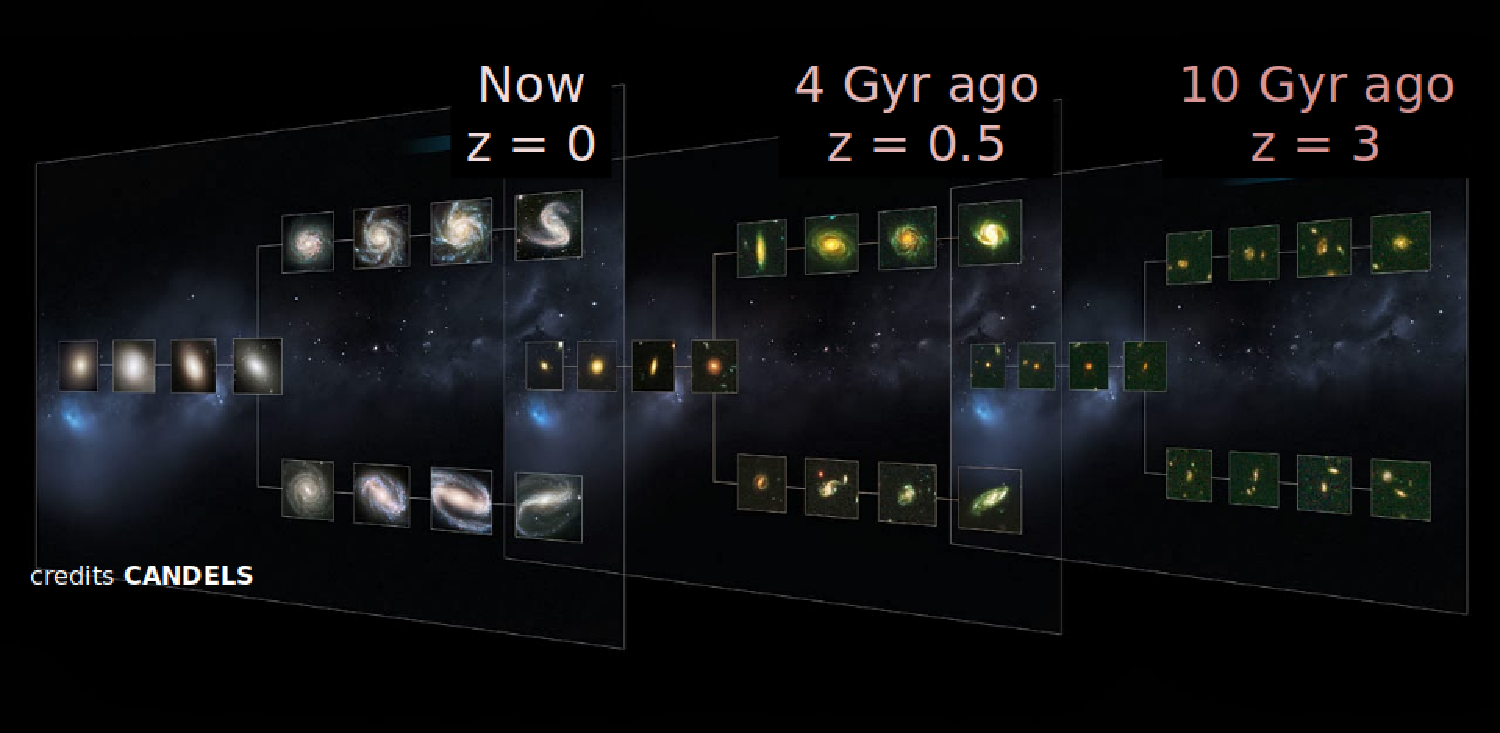
\includegraphics[width=\linewidth]{{graphics/evolution_gals}.pdf}

\end{frame}

\begin{frame}{Why studying kinematics ?}
	\begin{textblock*}{10cm}(1cm,1.66cm)
		\begin{tikzpicture}
			\useasboundingbox (0,-0.05) rectangle(\the\paperwidth,9.2);
			\fill[color=black] (-2,0+1.60) rectangle(\the\paperwidth,0.03+1.70);
	  	\end{tikzpicture}
  	\end{textblock*}
	
	\begin{textblock*}{10cm}(1.5cm, 1cm) 
		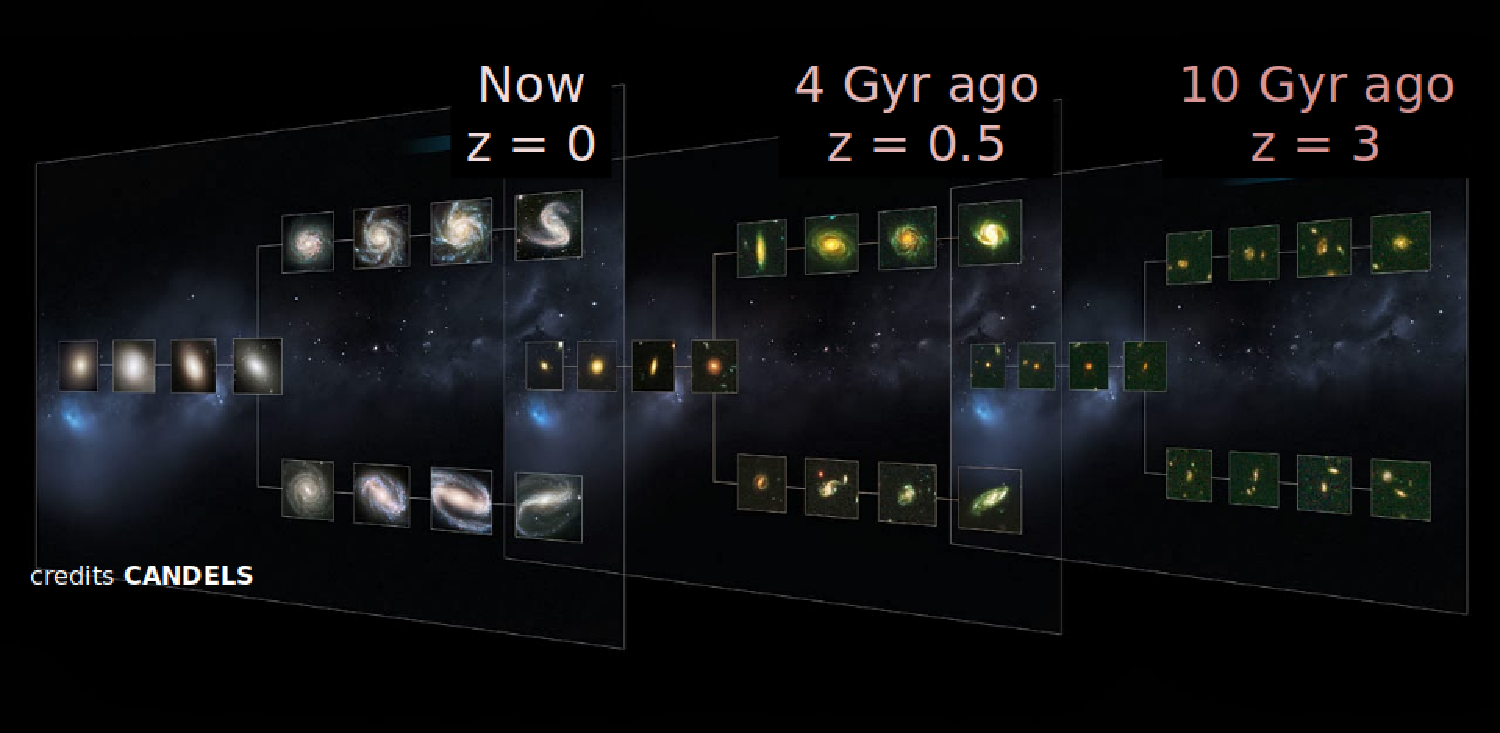
\includegraphics[width=\linewidth]{{graphics/evolution_gals}.pdf}
	\end{textblock*}
	
	\begin{textblock*}{11cm}(1cm, 5.8cm) 
		\color{white}
		Explain the co-evolution of morphological and dynamical properties of galaxies

		\begin{itemize}[label=$\rhd$]
			\item main processes responsible for disc formation and settling ?
			\item impact of merging, inflows and outflows on these processes ?
			\item kinematics $\rightarrow$ rotation curve $\rightarrow$ dark matter and angular momentum (re)distribution ?
		\end{itemize}
	\end{textblock*}
\end{frame}


\setbeamercolor{background canvas}{bg=white}
\color{black}
\begin{frame}{How ? }
	\framesubtitle{Kinematics data}
	
	\begin{columns}
		\begin{column}{0.7\linewidth}
			\underline{With IFS (MUSE):}
			\begin{itemize}[label=$\rhd$]
				\item \textbf{3D data cubes}
				\begin{enumerate}[label=(\alph*)]
					\item Measure galaxy redshifts
					\item Select spatially-resolved galaxies at intermediate redshift ($\mathbf{0.4 \lesssim z \lesssim 1.4}$)
					\item Ionised gas kinematics with \textbf{bright} (rest-frame) optical \textbf{emission lines} ($\rm{H}\beta$, [OII], [OIII], etc.)
				\end{enumerate}						
			\end{itemize}
			
			\begin{itemize}[label=+]
				\item Stellar kinematics now achievable for the brightest (m < 23) galaxies (Guérou+17)
			\end{itemize}
		\end{column}
		
		\begin{column}{0.48\linewidth}
			\hspace{-5pt}
			\vspace{-20pt}
			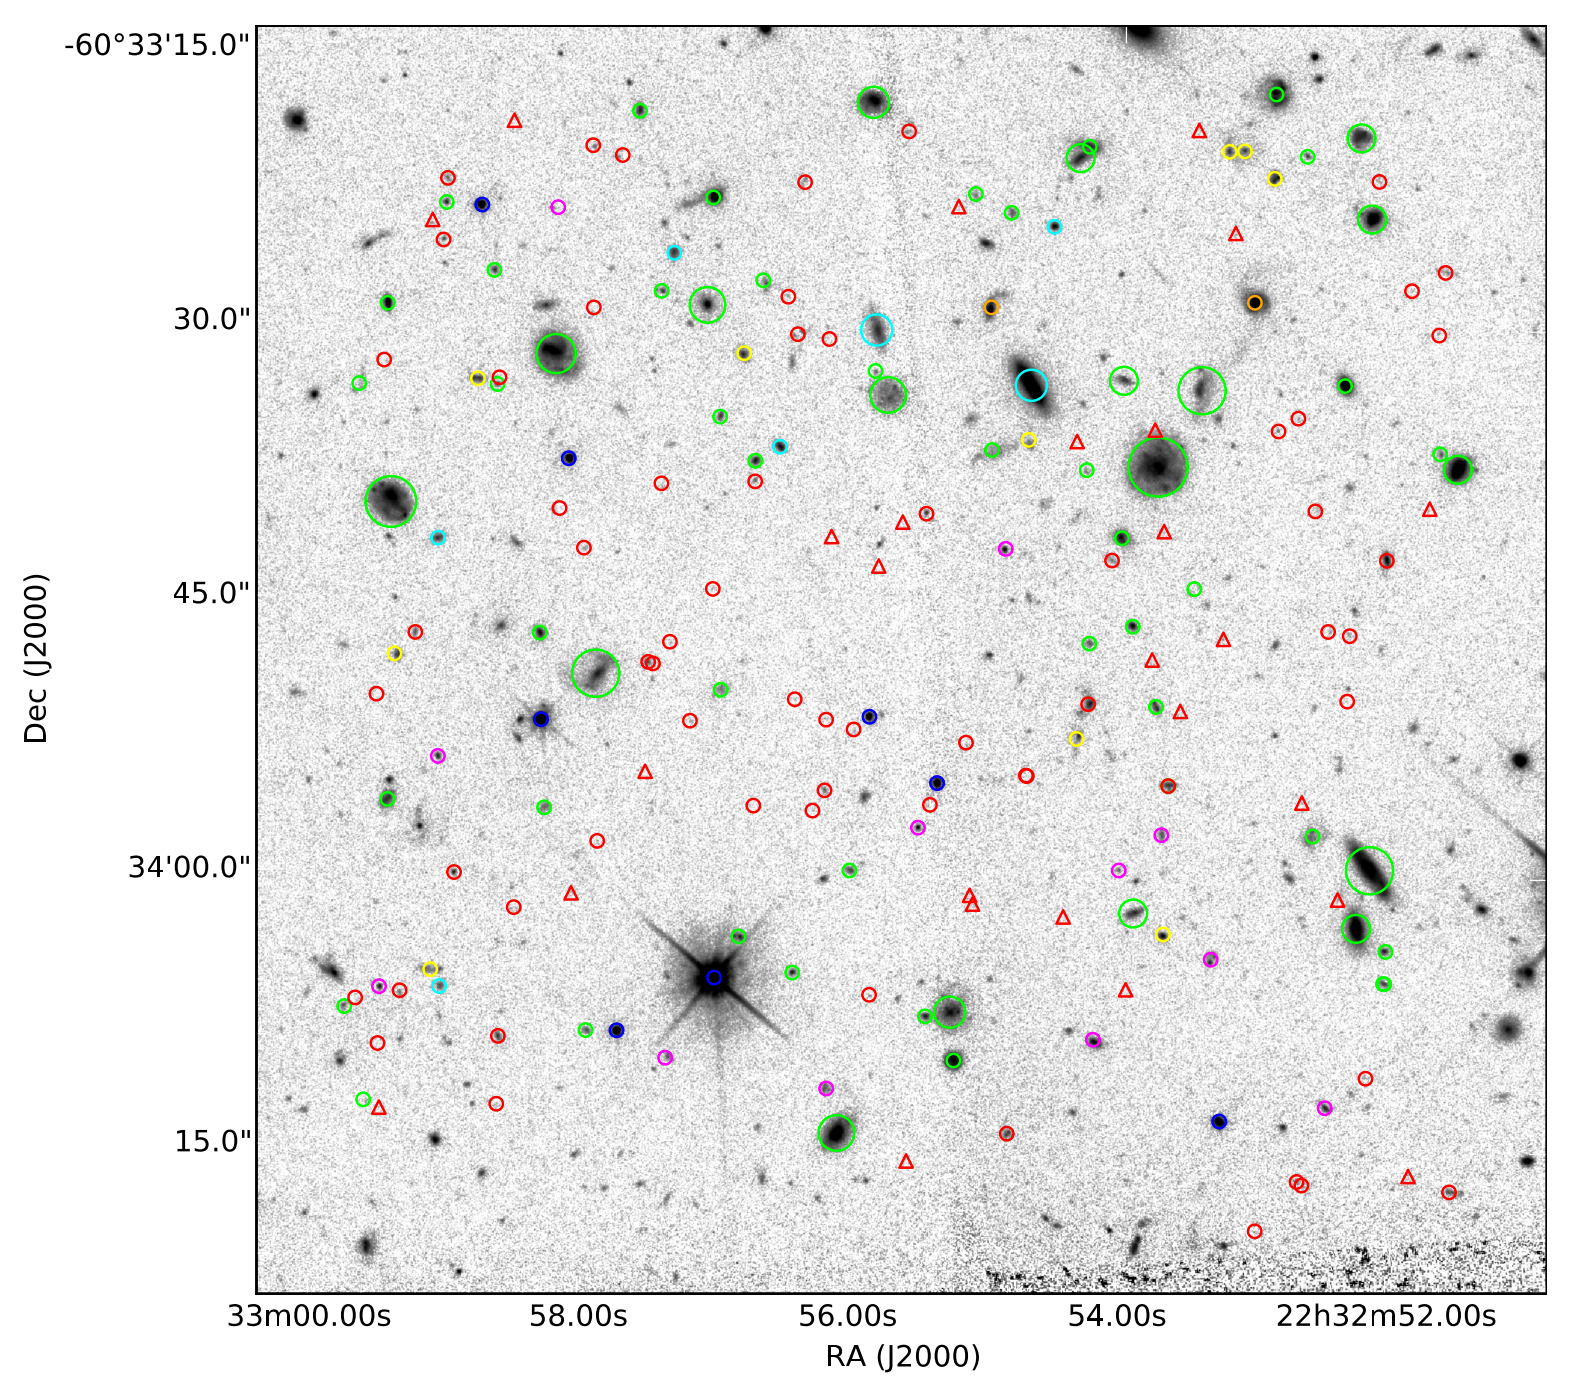
\includegraphics[width=\linewidth]{{graphics/HDFS}.png}
		\end{column}
	\end{columns}
	
	\vspace{-12pt}
	\hspace{58pt}
	\includegraphics[width=0.8\linewidth]{{graphics/spectrum_inami}.pdf}
	
	\begin{textblock*}{3.5cm}(4.3cm, 7.5cm)
		\textbf{\textcolor{orange}{Inami+17}}
	\end{textblock*}
	
	\begin{textblock*}{3.5cm}(10.3cm, 6cm)
		\textbf{\textcolor{orange}{Bacon+15}}
	\end{textblock*}
	
	\begin{textblock*}{3.5cm}(8.5cm, 2.8cm)
		\textbf{\textcolor{blue}{HDFS}}
	\end{textblock*}
\end{frame}




\begin{frame}{How ?}
	\framesubtitle{Kinematics data}
	\begin{columns}[T]
		\begin{column}{0.7\linewidth}
			\begin{itemize}[label=$\rhd$]
				\item Extract \textbf{2D maps} (\textcolor{orange}{flux}, \textcolor{blue}{velocity field} and \textcolor{red}{velocity dispersion})
				\begin{itemize}[label=$\circ$]
					\item Gaussian fit and rest-frame Doppler shift give LOS velocity (centroid) and velocity dispersion ($\rm{FWHM}$)
				\end{itemize}				
			\end{itemize}		
			
			\begin{figure}
				\vspace{9pt}
				\hspace{90pt}
				\centering
				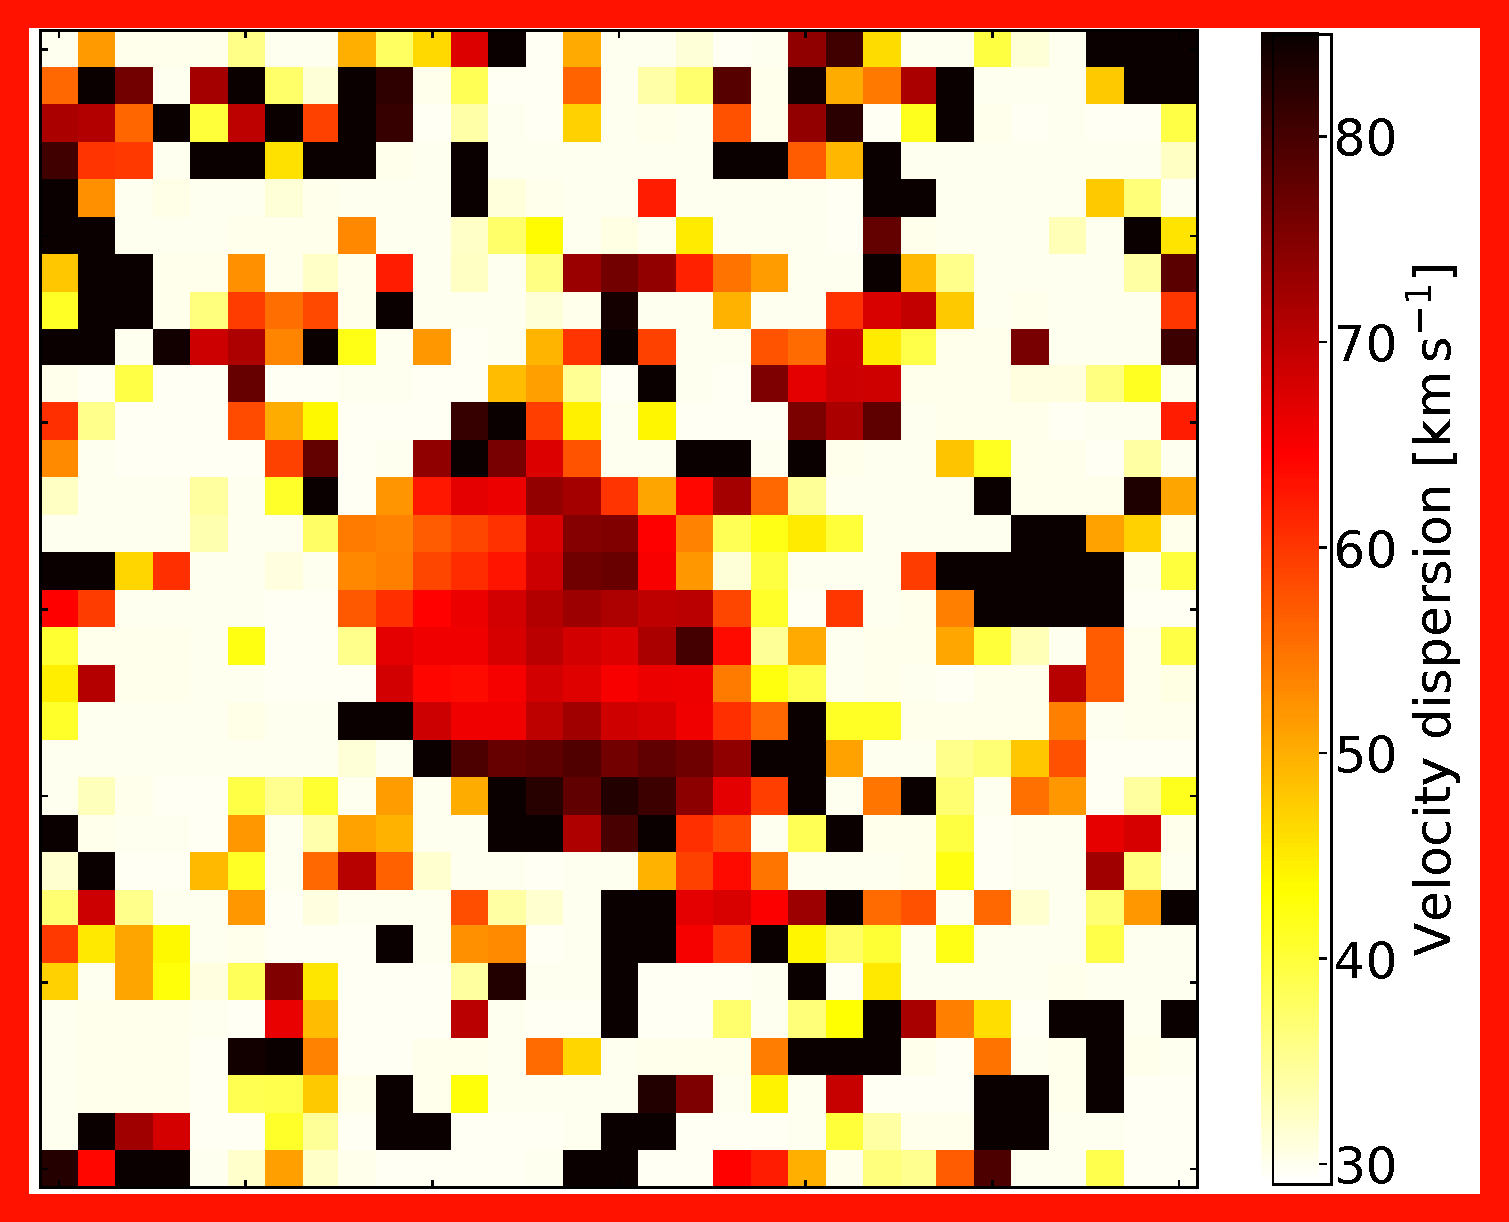
\includegraphics[width=0.55\linewidth]{{graphics/CGr30bs_139_disp_cadre}.pdf}
			\end{figure}		
		\end{column}

		\begin{column}{0.4\linewidth}
			\begin{figure}
				\vspace{-15pt}
				\centering
				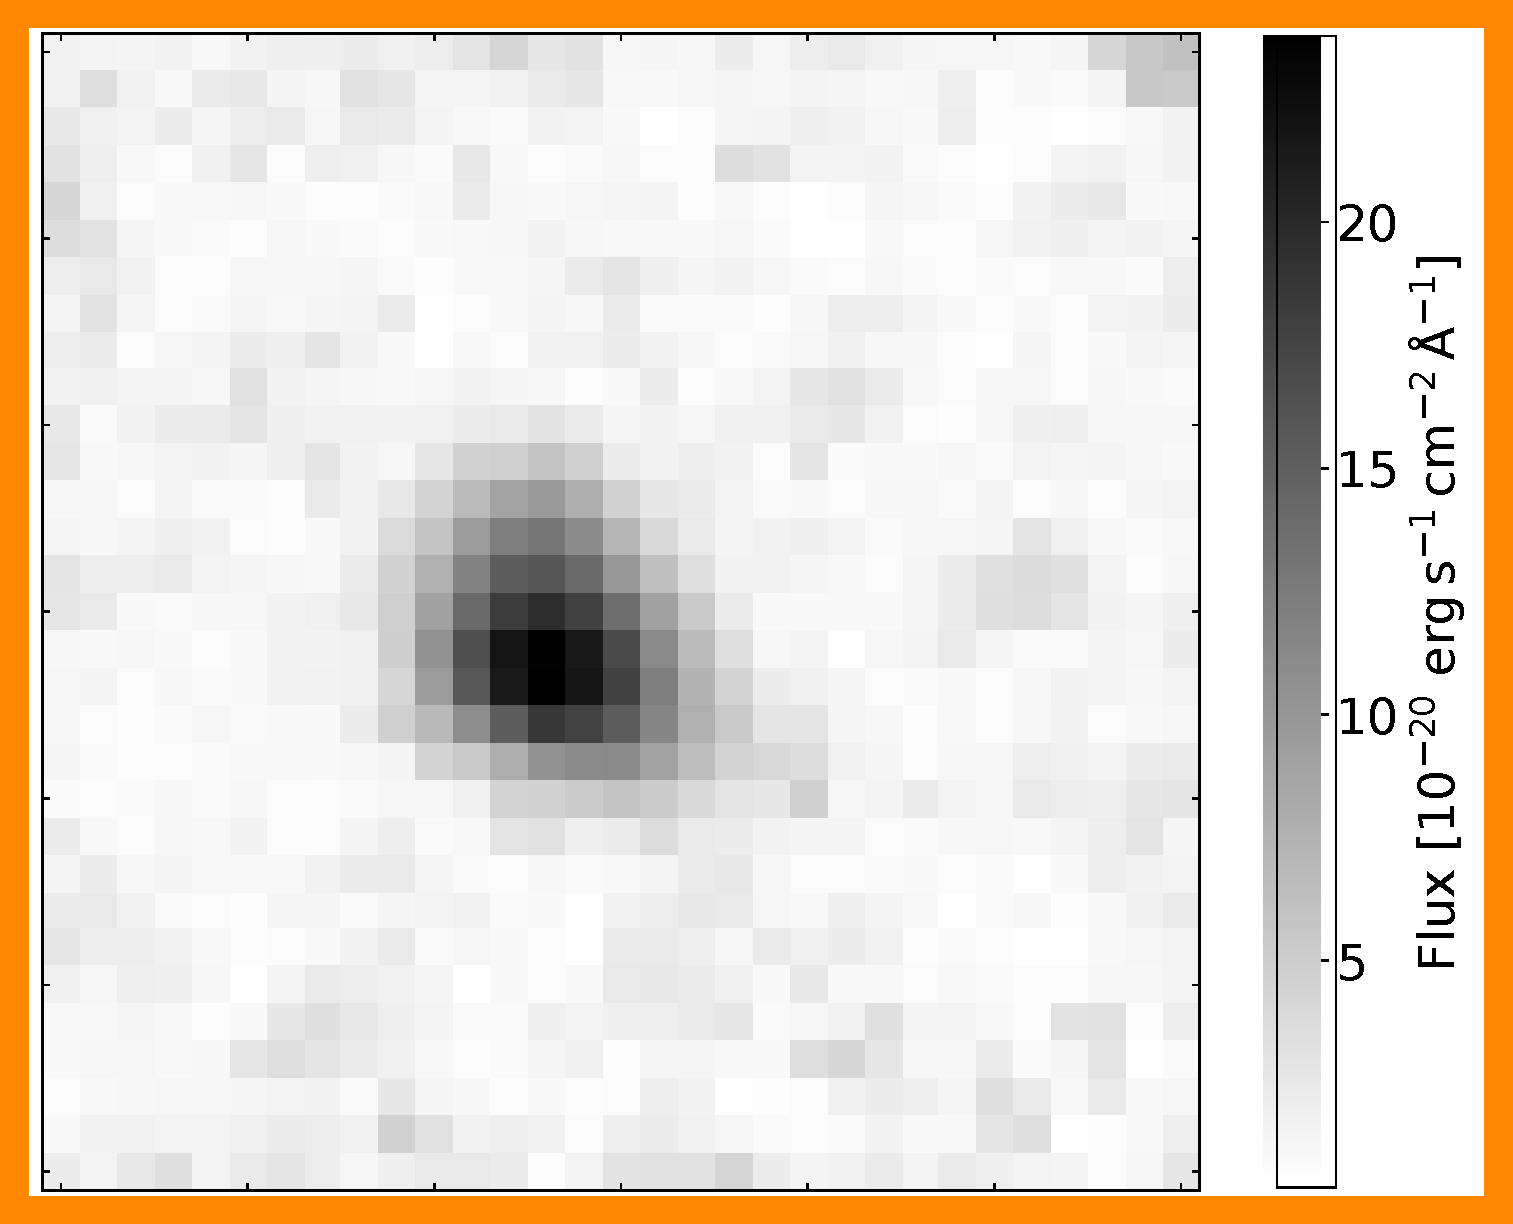
\includegraphics[width=\linewidth]{{graphics/CGr30bs_139_flux_cadre}.pdf}
				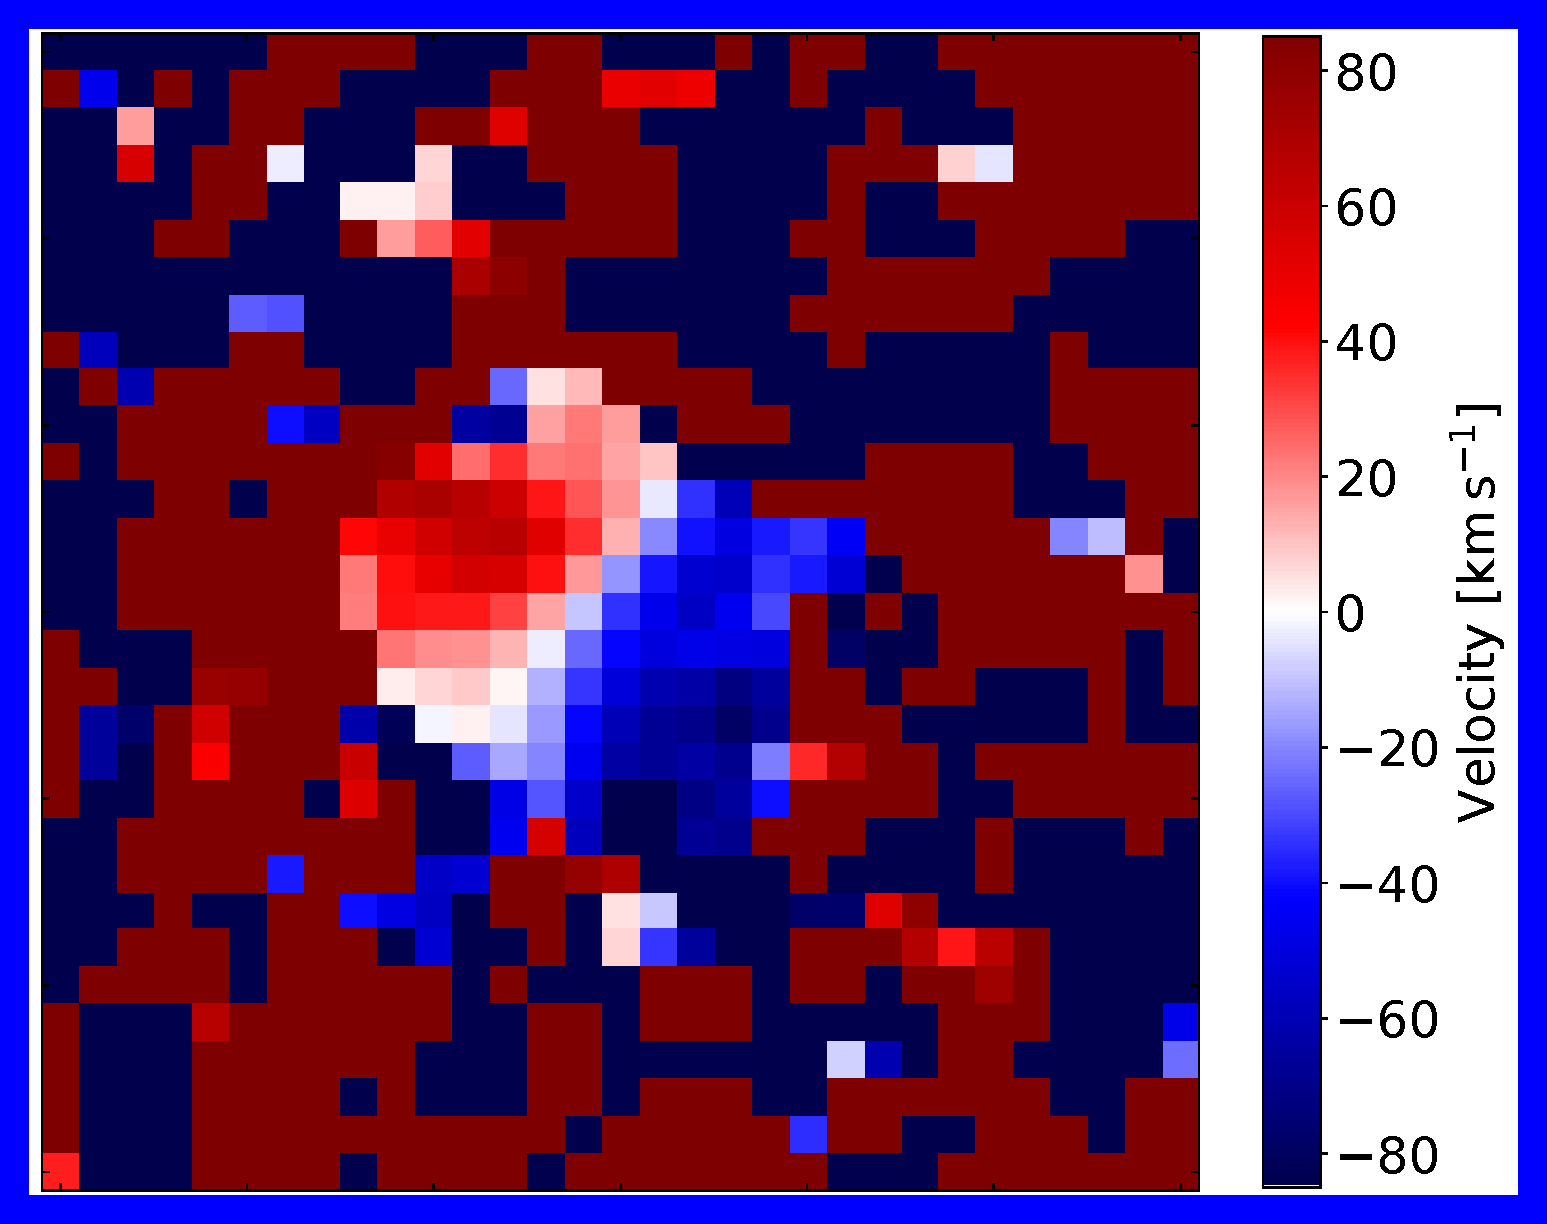
\includegraphics[width=\linewidth]{{graphics/CGr30bs_139_vel_cadre}.pdf}
			\end{figure}
		\end{column}
	\end{columns}
	
	\begin{textblock*}{3.5cm}(8.3cm, 1.9cm)
		{\tiny CGr30bs\_139 \\ \vspace{-5pt}($z \approx 0.7$)}
	\end{textblock*}
\end{frame}

\begin{frame}{How ?}
	\framesubtitle{Modelling}
	\begin{columns}[T]
		\begin{column}{0.8\linewidth}
			\vspace{-10pt}
			\begin{itemize}[label=$\rhd$]
				\item $\sigma_{\rm{v}}$ \textbf{overestimated} $\rightarrow$ PSF and LSF must \\ be taken into account (beam smearing) 
				
				\item Need for ancillary data (high-res images, galaxies inclination and size, etc.)
				\begin{itemize}[label=$\circ$]
					\item  inclination required for modelling ($V_{\rm{obs}} \propto \sin i$)
				\end{itemize}	
			\end{itemize}
			
			\begin{figure}
				\centering
				\vspace{-10pt}
				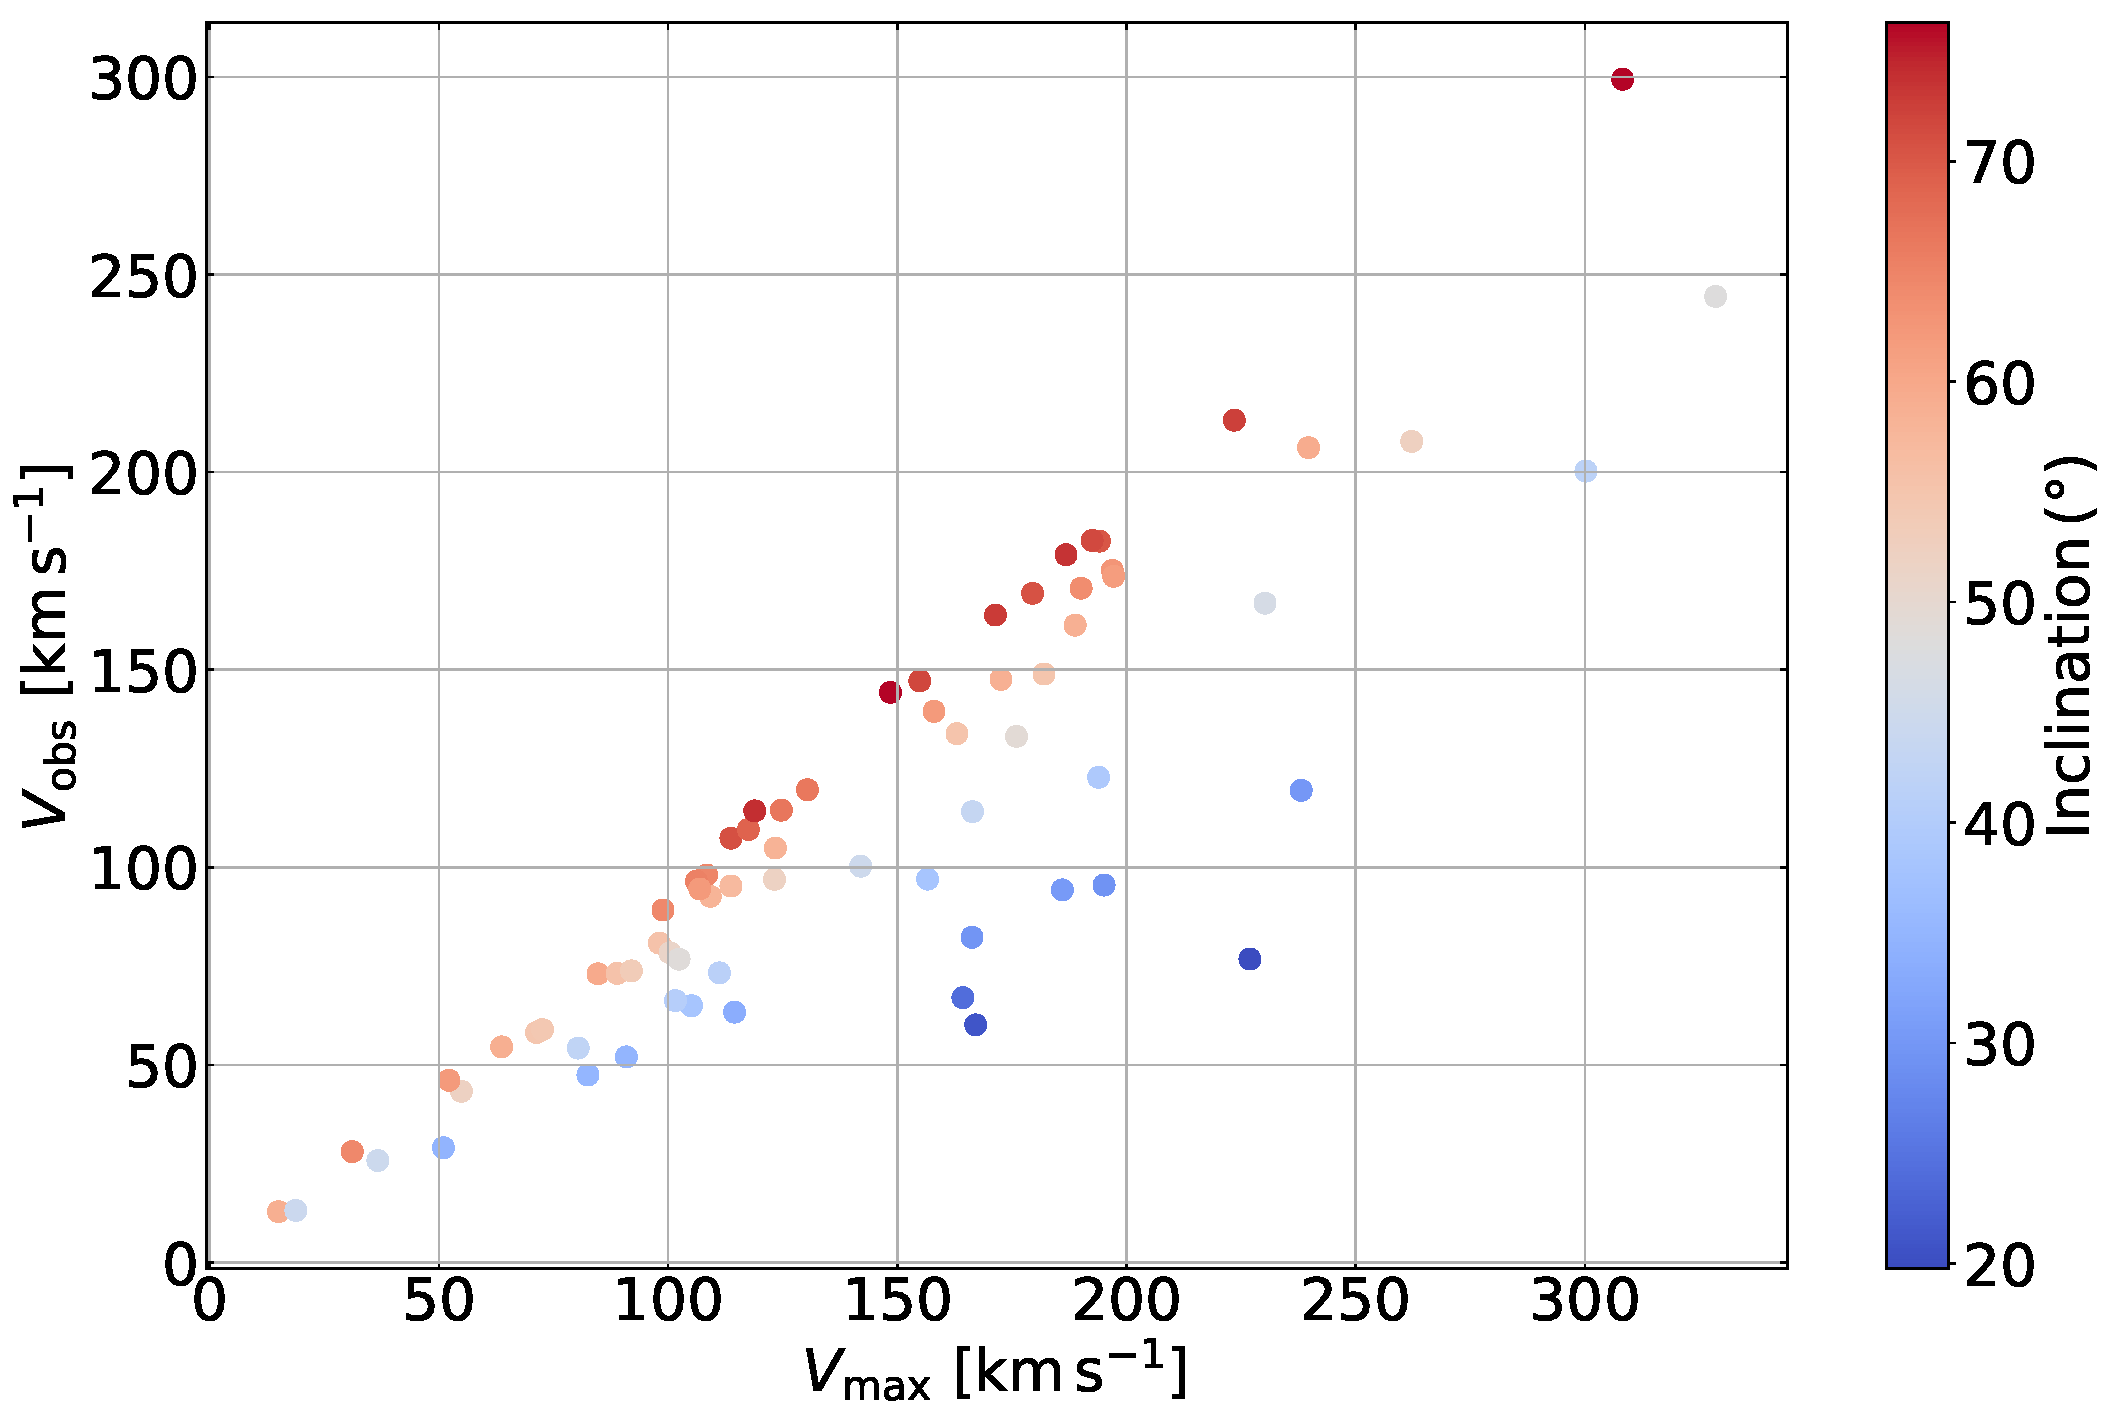
\includegraphics[width=0.8\linewidth]{{graphics/effect_of_inclination}.pdf}
			\end{figure}					
		\end{column}

		\hspace{-15pt}
		\begin{column}{0.4\linewidth}
			\begin{figure}
				\vspace{-15pt}
				\centering
				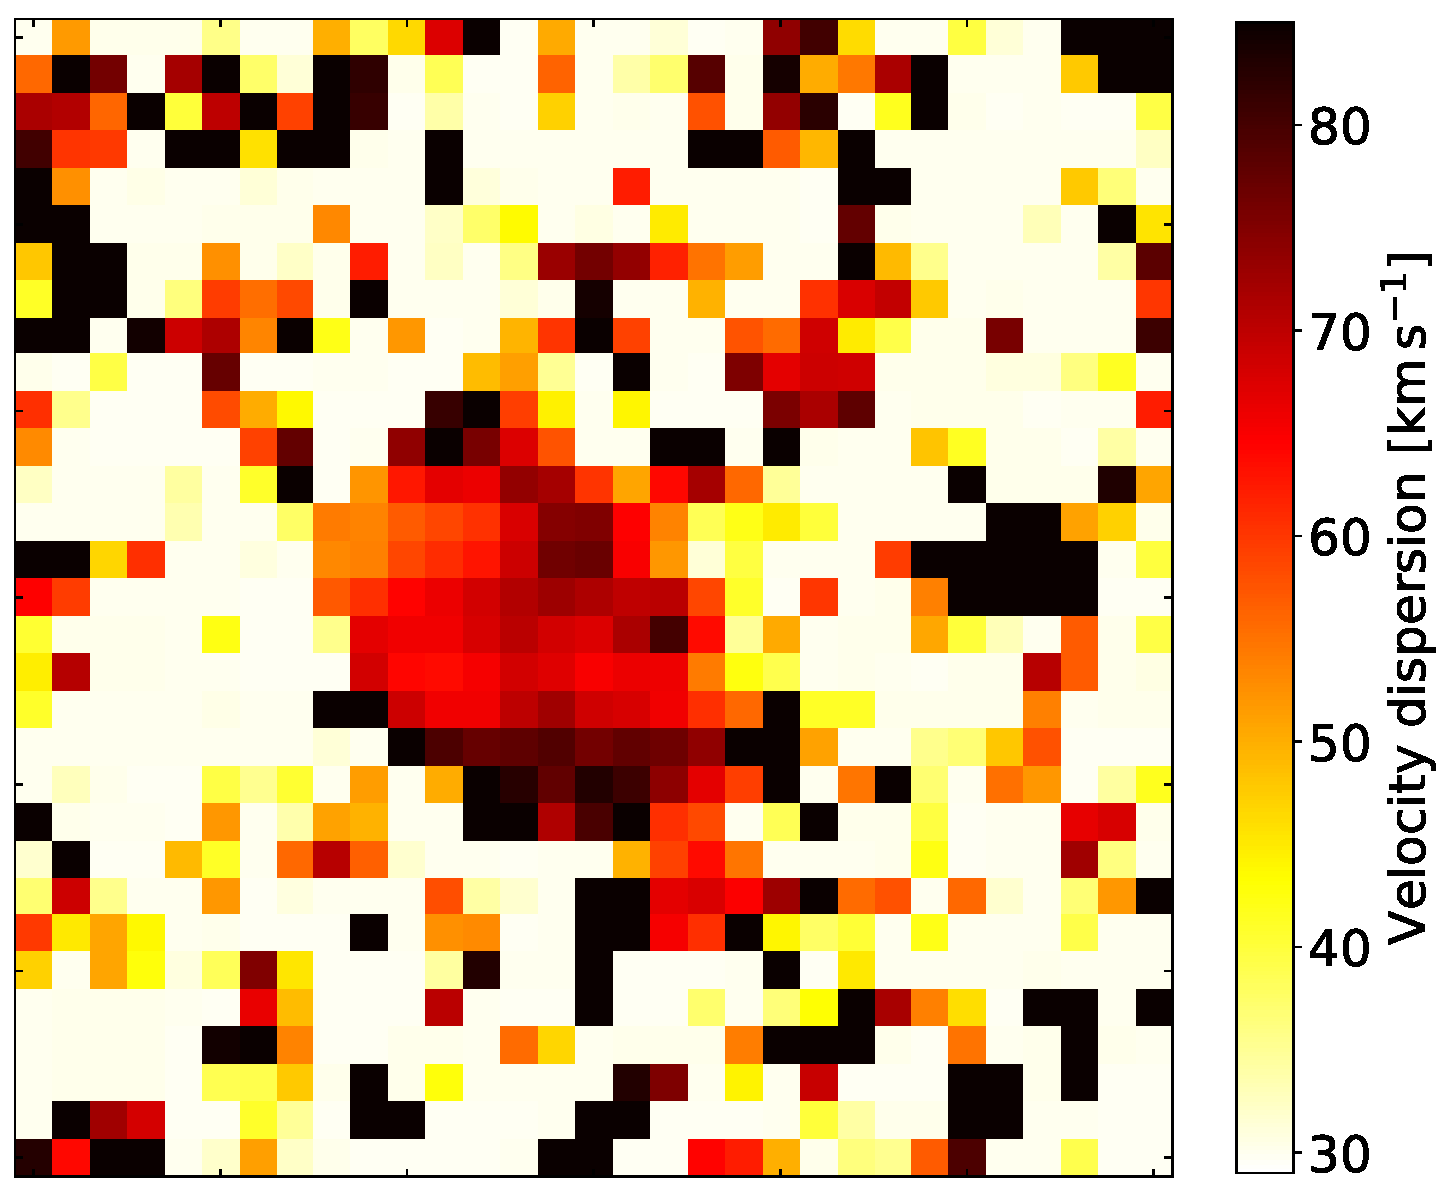
\includegraphics[width=\linewidth]{{graphics/CGr30bs_139_disp}.pdf}
				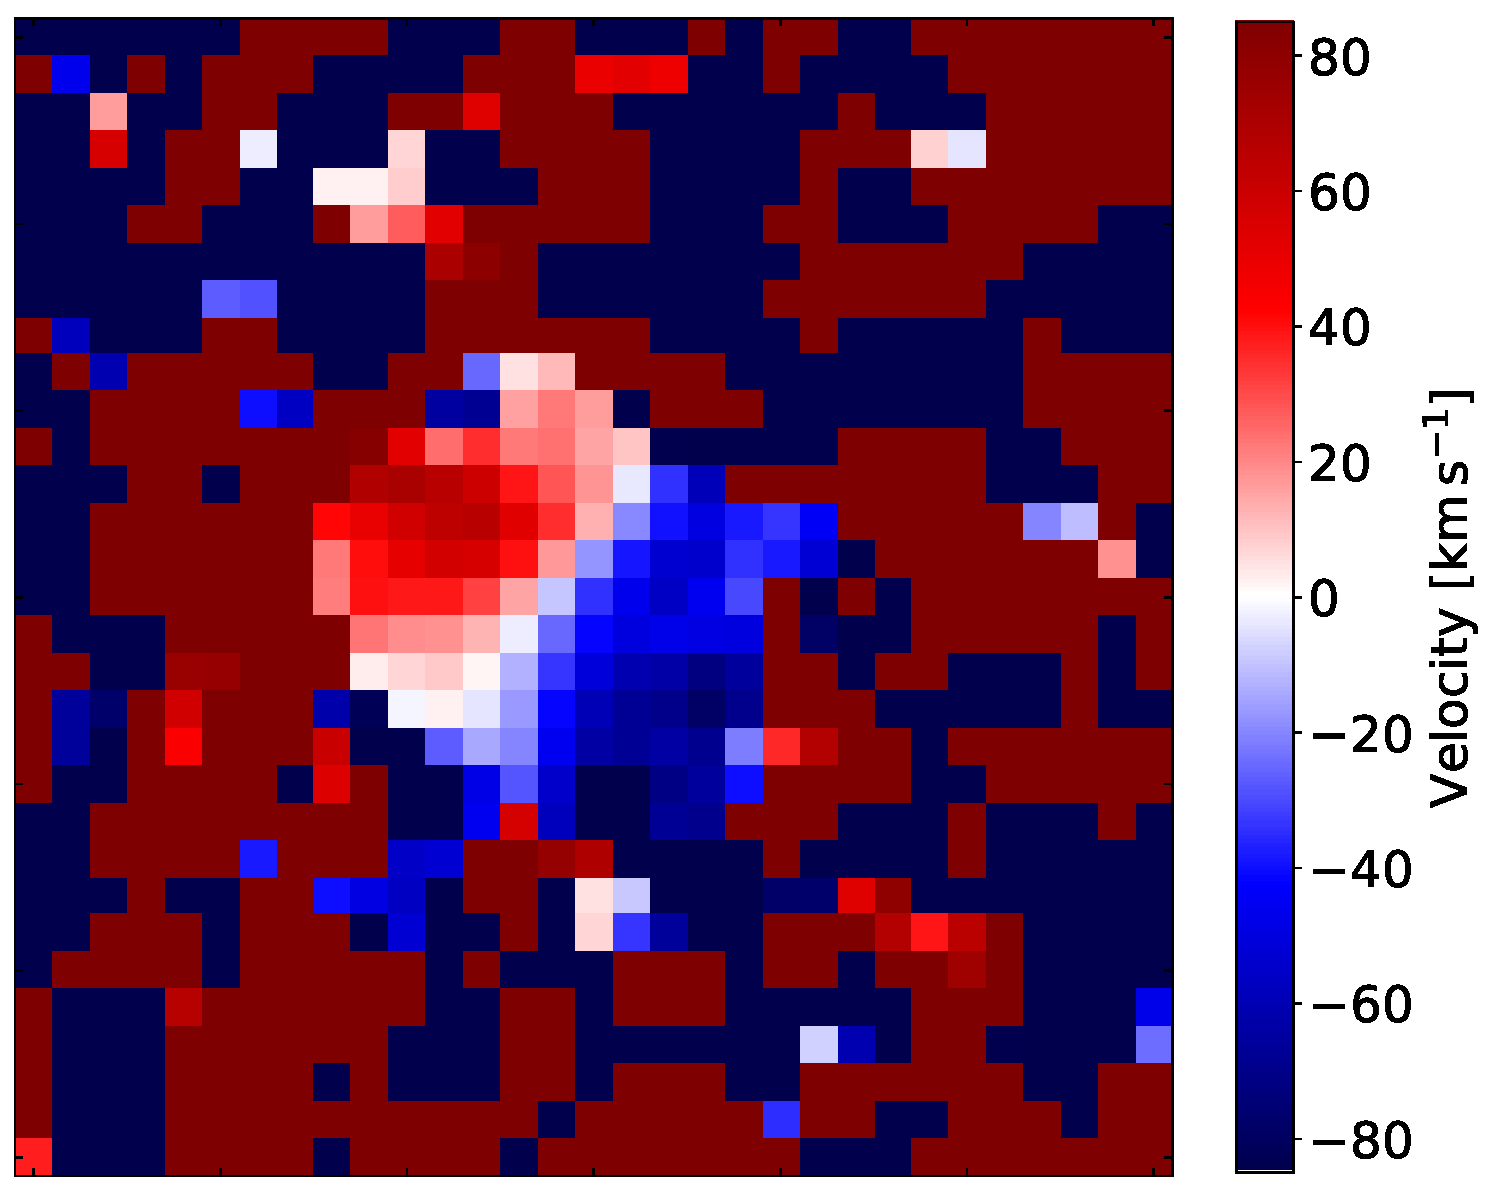
\includegraphics[width=\linewidth]{{graphics/CGr30bs_139_vel}.pdf}
			\end{figure}
		\end{column}
	\end{columns}
\end{frame}



\begin{frame}{How ?}
	\framesubtitle{Modelling: two different methods}
	\begin{columns}[T]
		\begin{column}{\linewidth}
			
			\underline{2D fitting:}
			\begin{itemize}[label=$\rhd$]
				\item Works with 2D velocity field and dispersion assuming either
				
			\begin{enumerate}[label=(\alph*)]
				\item a \textbf{mass distribution} (can describe declining curves at large radius)
				\item a \textbf{fixed function} (arctan, \textbf{ramp model}, etc.) which describes the  observed flattening of curves
			\end{enumerate}
				
			\end{itemize}
			
			\vfill
			
			\underline{3D fitting:}
			\begin{itemize}[label=$\rhd$]
				\item improvement for faint and compact galaxies
				
				\begin{itemize}[label=$\circ$]
					\item GALPAK\textsuperscript{3D} (Bouché+15)
					\item \textsuperscript{3D}BAROLO (Di Teodoro \& Fraternali+15)
				\end{itemize}
			\end{itemize}		
		\end{column}
	\end{columns}
\end{frame}



\section{Initial sample}
\begin{frame}{Application to my internship}
	\framesubtitle{Initial sample}
	\begin{columns}
		\begin{column}{0.65\linewidth}	
			\begin{figure}
				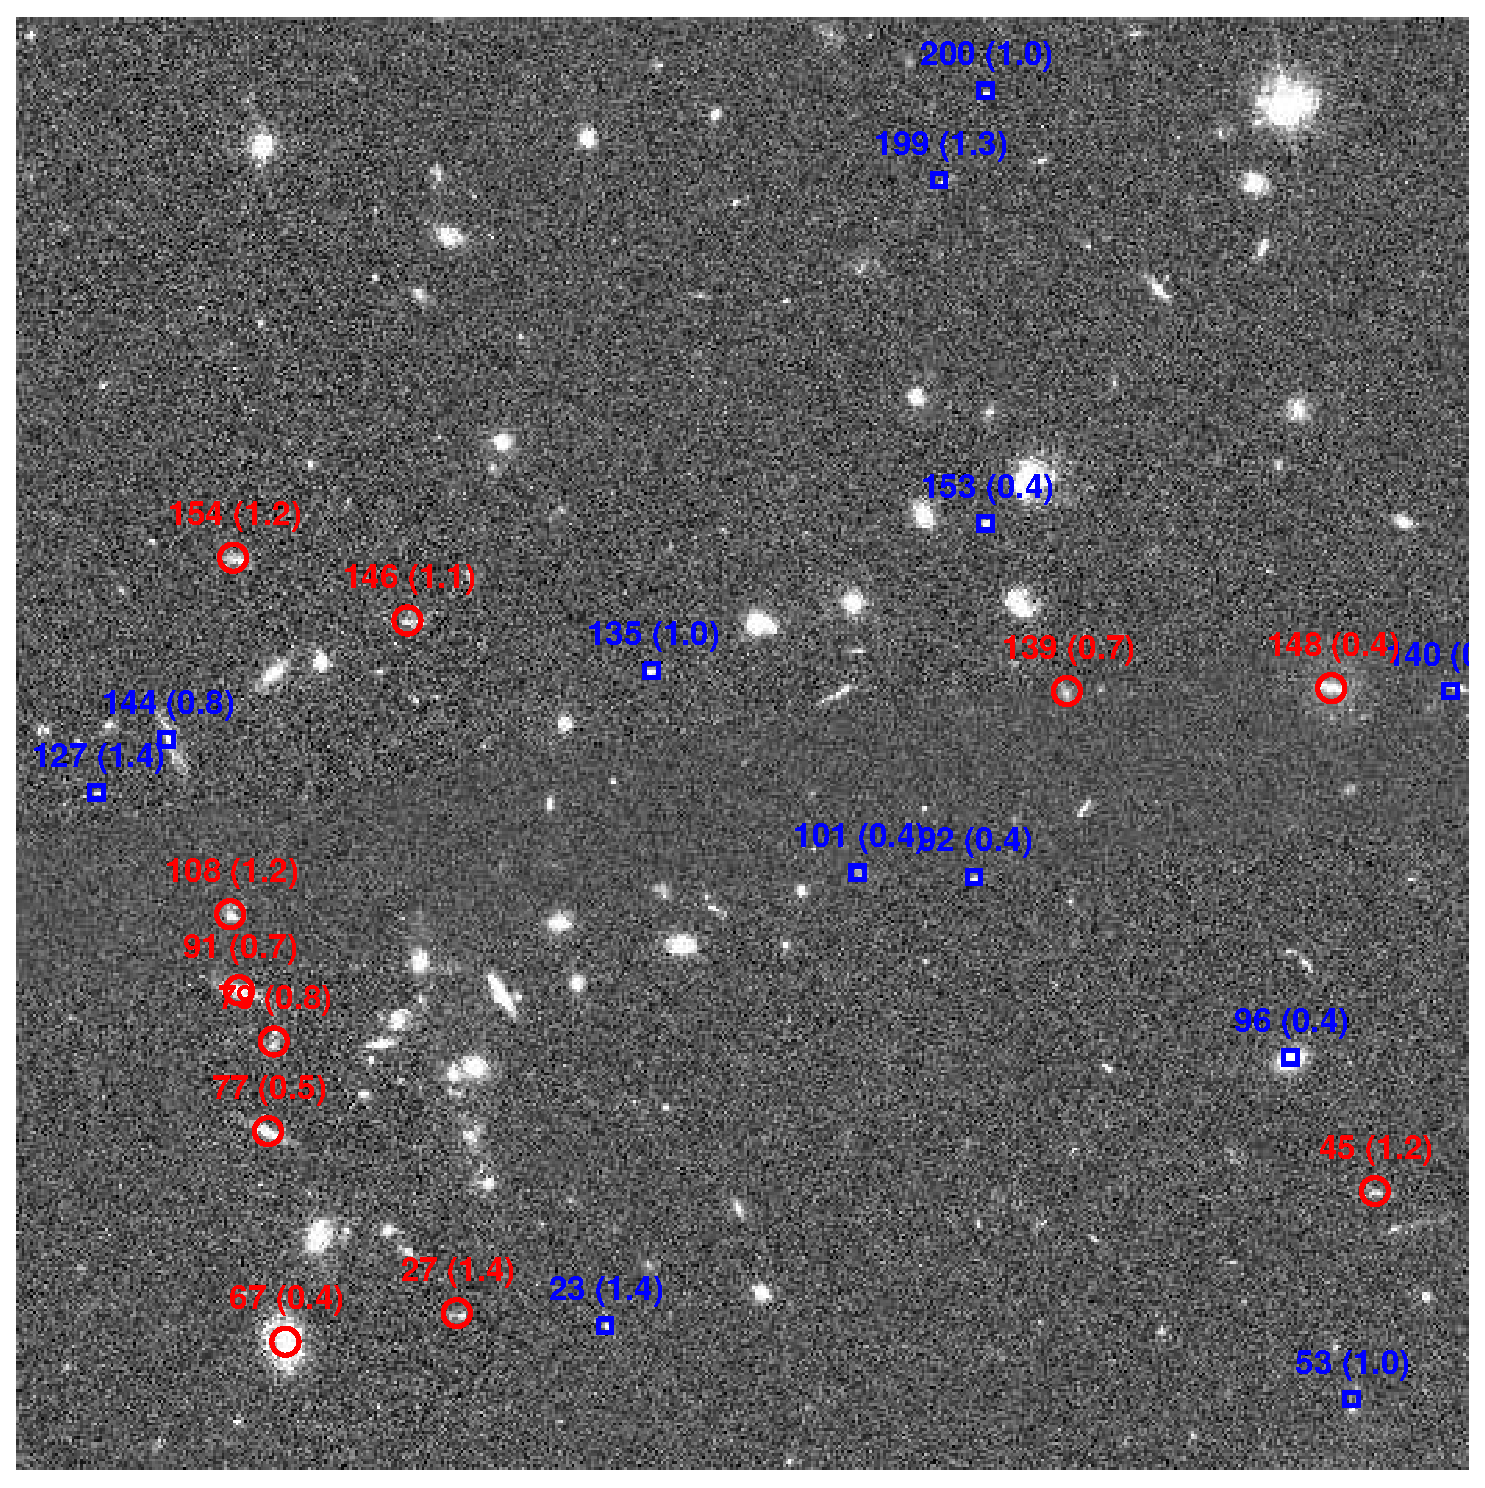
\includegraphics[width=\linewidth]{{graphics/CGr30}.eps}
				\caption{HST image of COSMOS group CGr30}
			\end{figure}
		\end{column}
		
		\hspace{-10pt}
		\begin{column}{0.5\linewidth}
			\begin{itemize}[label=$\rhd$]
				\item $16$ MUSE fields in COSMOS area
				\item exposures from $1$ to $\SI{10}{hr}$
				\item seeing-limited ($\rm{FWHM} \lesssim \SI{0.7}{"}$) or AO ($\rm{FWHM} \lesssim \SI{0.5}{"}$)
				\item $\mathbf{\sim 500}$ \textbf{field galaxies with [OII] detection}
				\begin{itemize}[label=$\cdot$]
					\item HST-ACS counterparts
					\item $\mathbf{0.4 \leq z \leq 1.4}$
				\end{itemize}
			\end{itemize}
		\end{column}
	\end{columns}
\end{frame}


\section{Internship methodology}
\subsection{Methodology}
\begin{frame}{Methodology}
	\begin{textblock*}{11.5cm}(0.1cm, 1.2cm)
		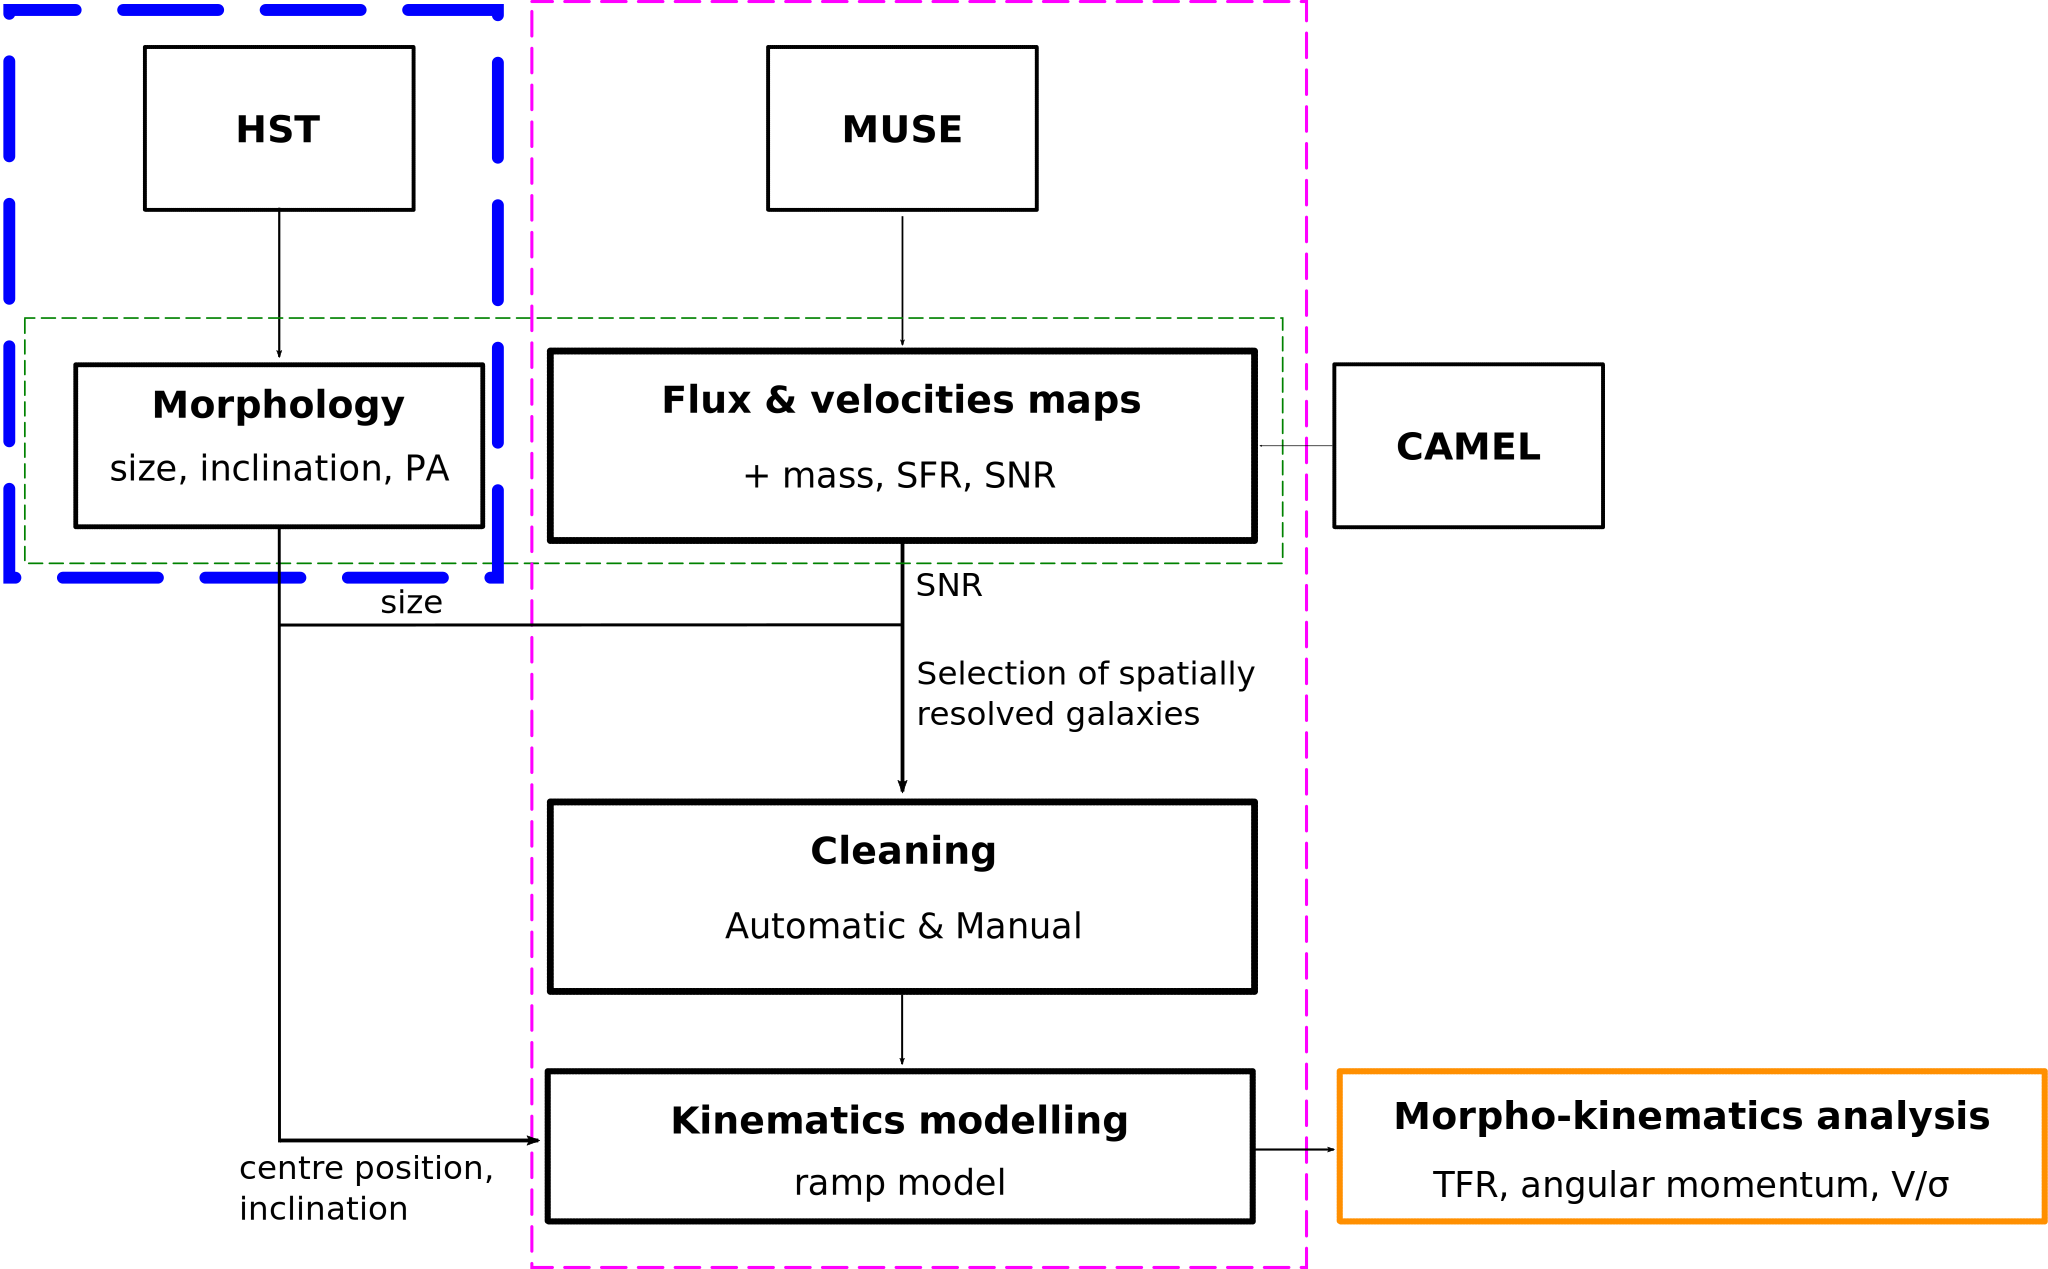
\includegraphics[width=1.1\linewidth]{{graphics/SchematicsMorpho}.eps}
	\end{textblock*}
	
	\begin{textblock*}{11cm}(8.5cm, 5cm)
		\textcolor{OliveGreen}{Prior data/information} \\ 
		{\Large\textbf{\textcolor{blue}{Morphology}}} \\ 
		\textcolor{magenta}{Kinematics} \\ 
		\textcolor{orange}{Analysis}
	\end{textblock*}
	
\end{frame}



\begin{frame}{Selection of a sample of spatially resolved galaxies}
	\vspace{-3pt}
	
	%drawing first circle (red)
	\begin{textblock*}{5cm}(8.5cm,4cm)
		\begin{tikzpicture}
    		\draw [red, rotate=25] (0,0) ellipse (0.8cm and 2.2cm);
		\end{tikzpicture}	
	\end{textblock*}
	
	%drawing second circle (blue)
	\begin{textblock*}{5cm}(5.6cm,4.4cm)
		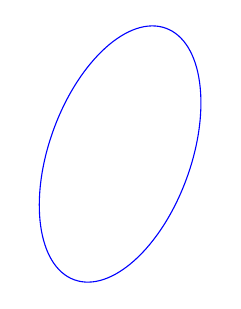
\begin{tikzpicture}
    		\draw [blue, rotate=-20] (0,0) ellipse (0.9cm and 1.7cm);
		\end{tikzpicture}	
	\end{textblock*}
	
	\begin{columns}
		\begin{column}{0.4\linewidth}
			\begin{itemize}[label=$\rhd$]				
				\item Most of our sample galaxies are on the main sequence
				\item \textcolor{red}{massive quiescent} (low [OII]) and \textcolor{blue}{very low mass galaxies} (small size) are lost
			\end{itemize}
			
			\begin{figure}
				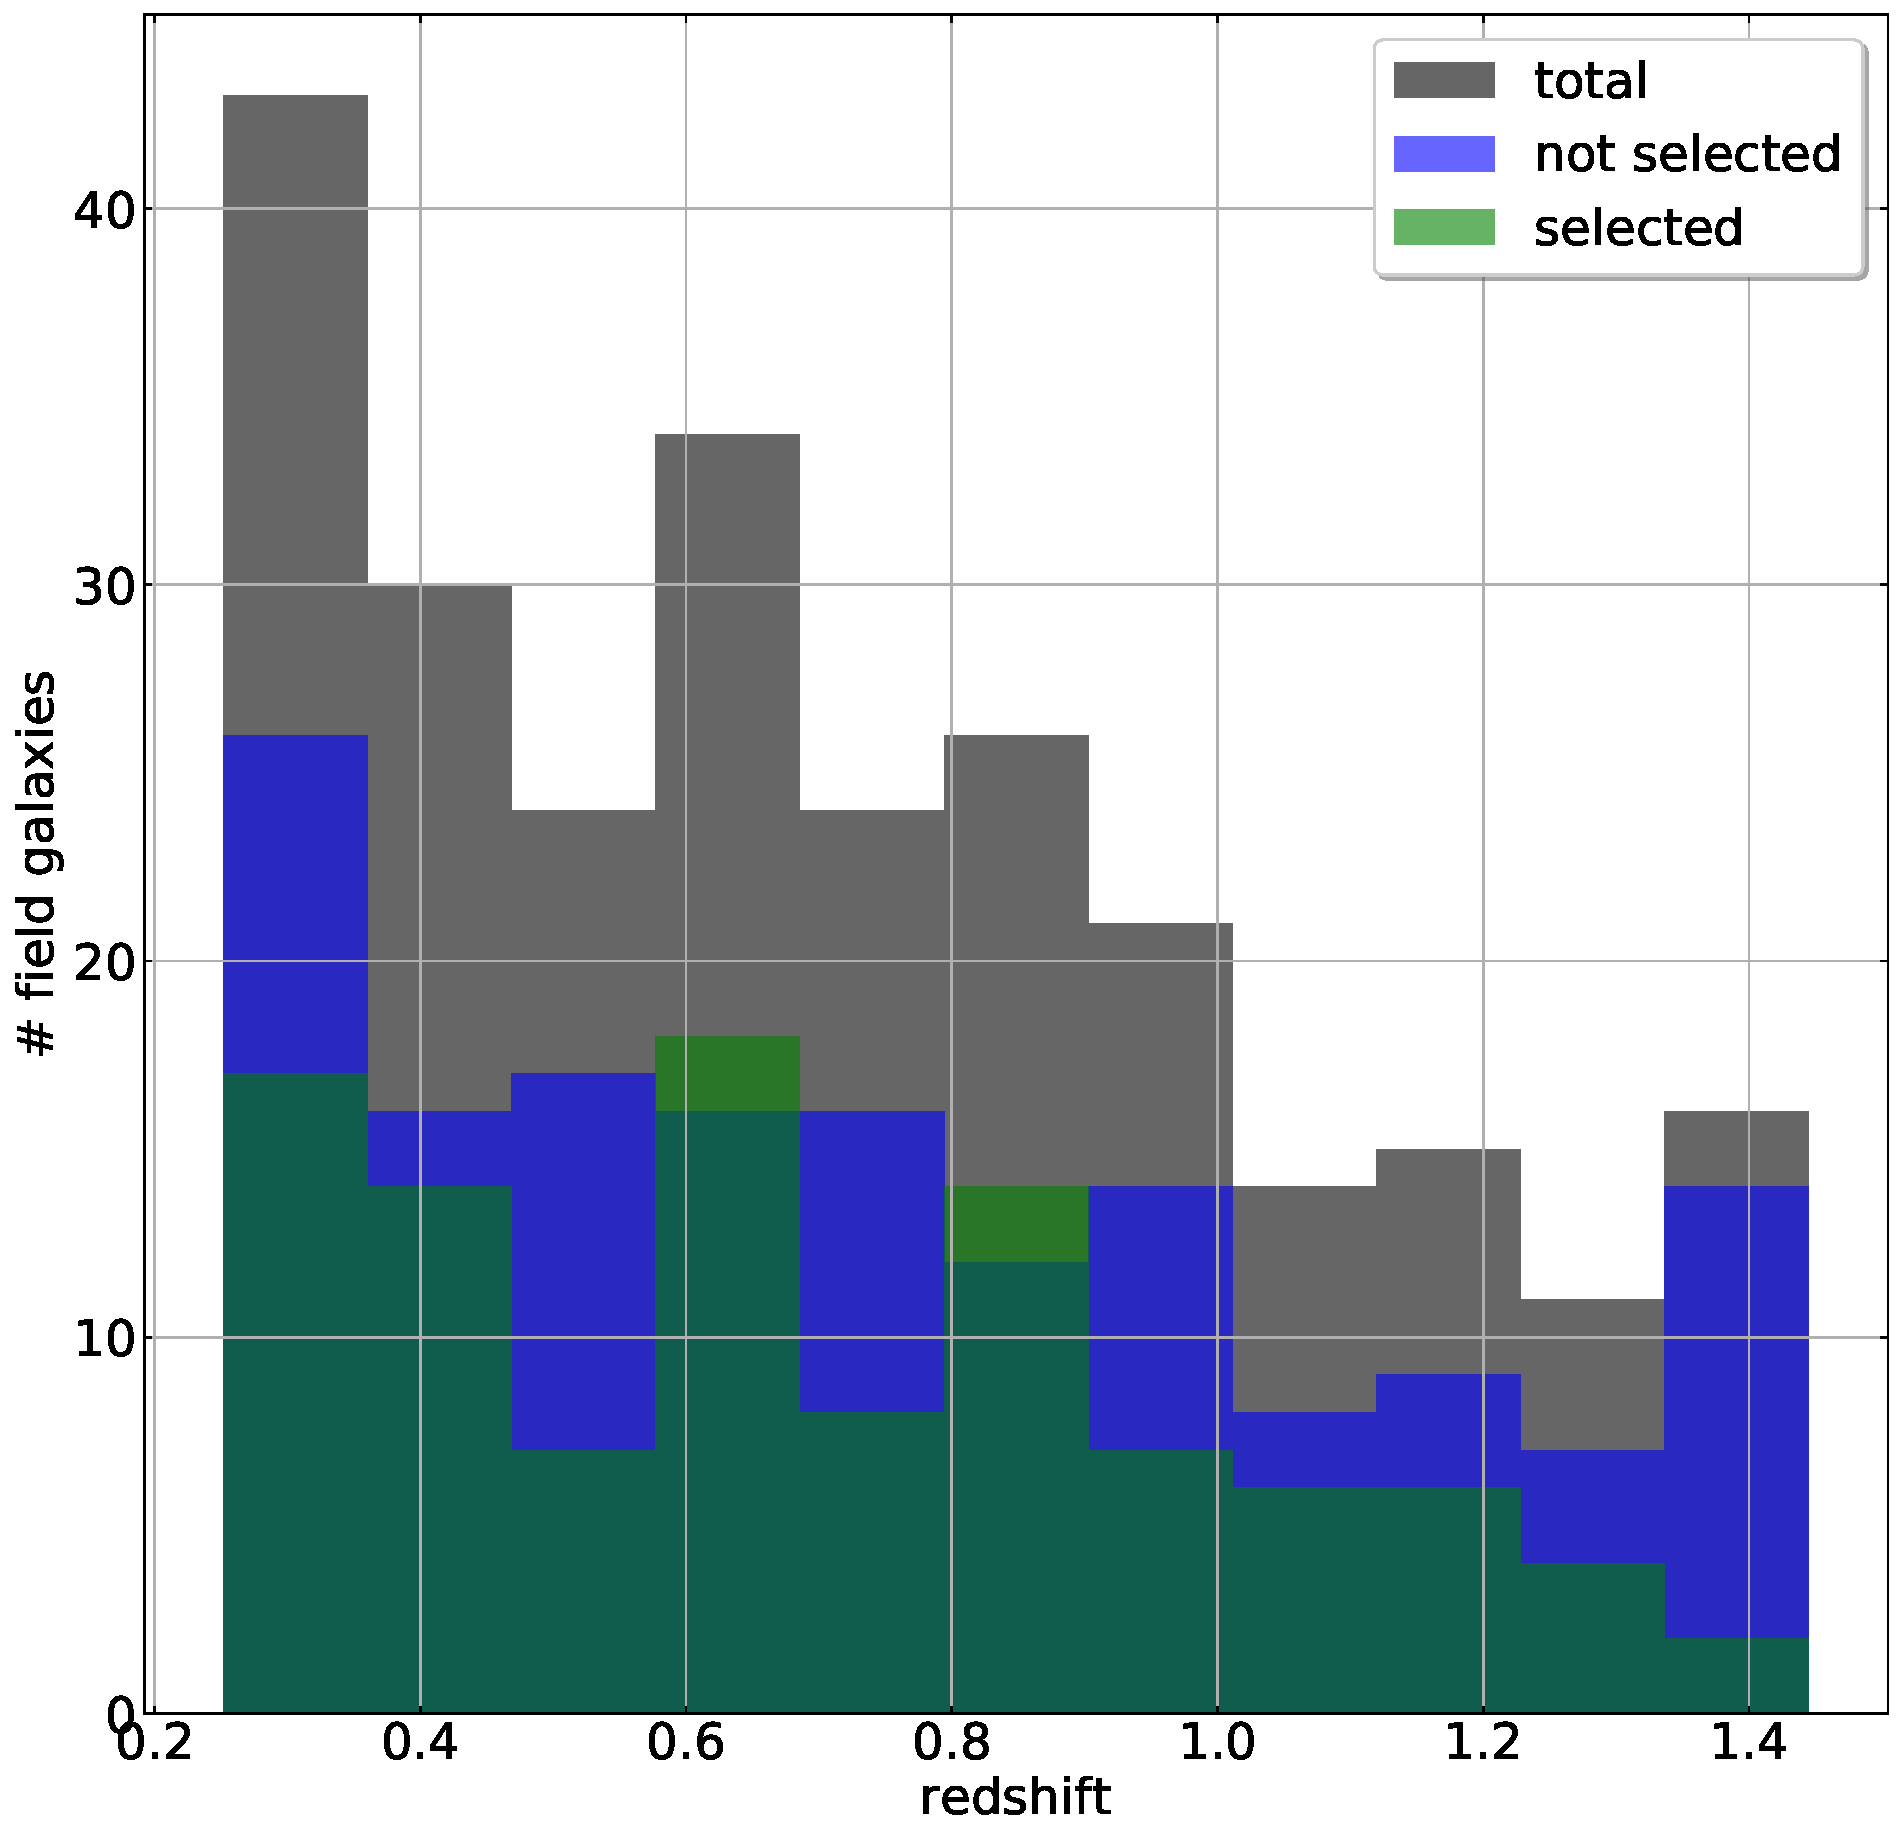
\includegraphics[width=0.9\linewidth]{{graphics/hist_redshift}.pdf}			
			\end{figure}
			
		\end{column}
		\begin{column}{0.75\linewidth}
		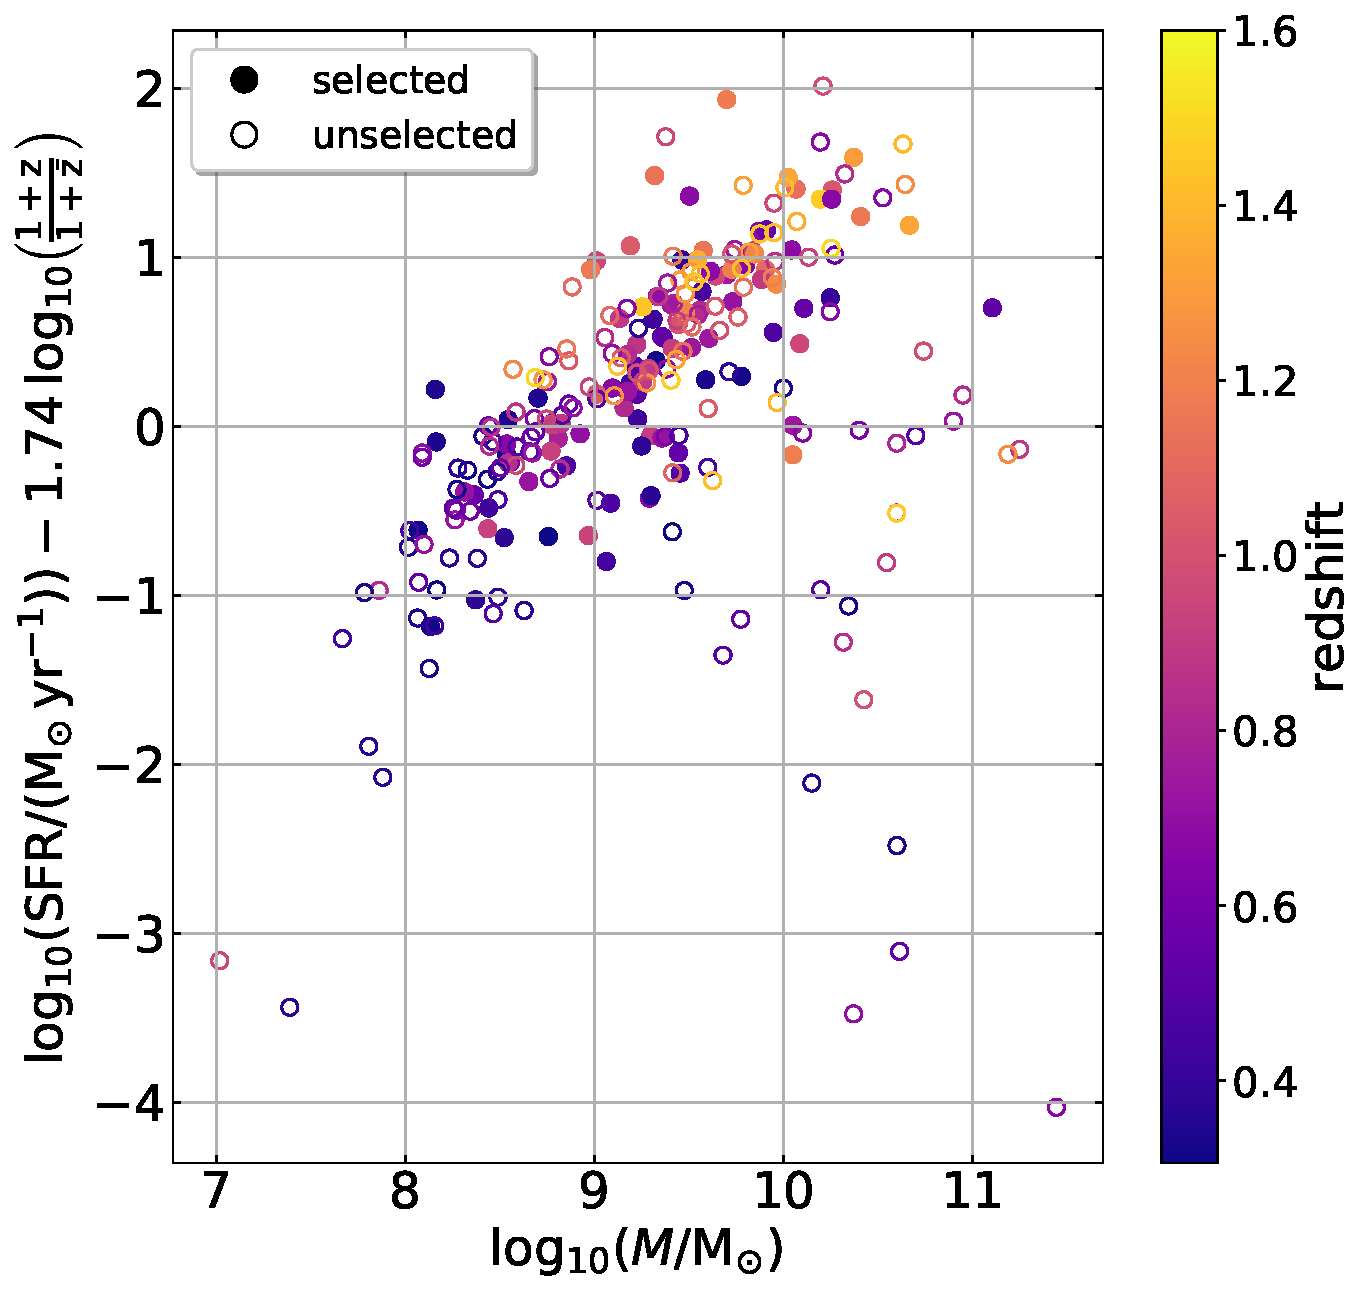
\includegraphics[width=\linewidth]{{graphics/SFR_vs_mass_correctedversiononly}.pdf}
		\end{column}
	\end{columns}		
\end{frame}

\section{Methodology}
\subsection{Methodology}
\begin{frame}{Methodology}
	\begin{textblock*}{11.5cm}(0.1cm, 1.2cm)
		
\includegraphics[width=1.1\linewidth]{{graphics/SchematicsKinematics}.eps}
	\end{textblock*}
	
	\begin{textblock*}{11cm}(8.5cm, 5cm)
		\textcolor{OliveGreen}{Prior data/information} \\ 
		\textcolor{blue}{Morphology} \\ 
		{\Large\textbf{\textcolor{magenta}{Kinematics}}} \\ 
		\textcolor{orange}{Analysis}
	\end{textblock*}
	
\end{frame}

\section{Kinematical modelling}
\subsection{Cleaning galaxies}
\begin{frame}{Kinematical modelling}
	\framesubtitle{Cleaning galaxies}
	\begin{columns}	
		\begin{column}{0.6\linewidth}
			\vspace{100pt}		
			\centering
			
\includegraphics[width=0.5\linewidth]{{graphics/VelBefore}.eps}
		\end{column}

		\begin{column}{0.6\linewidth}
			\vspace{100pt}		
			\centering
			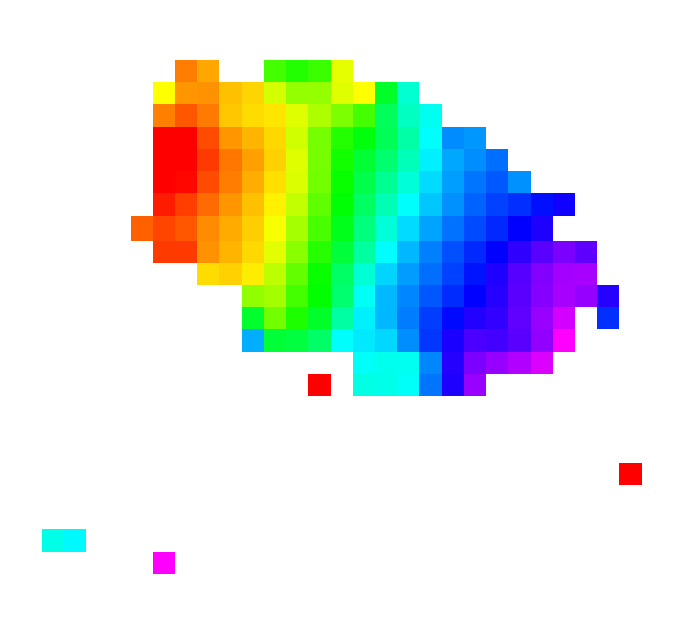
\includegraphics[width=0.5\linewidth]{{graphics/VelAuto}.eps}
		\end{column}
	\end{columns}
	
	\begin{textblock*}{5cm}(8.5cm,6cm)
		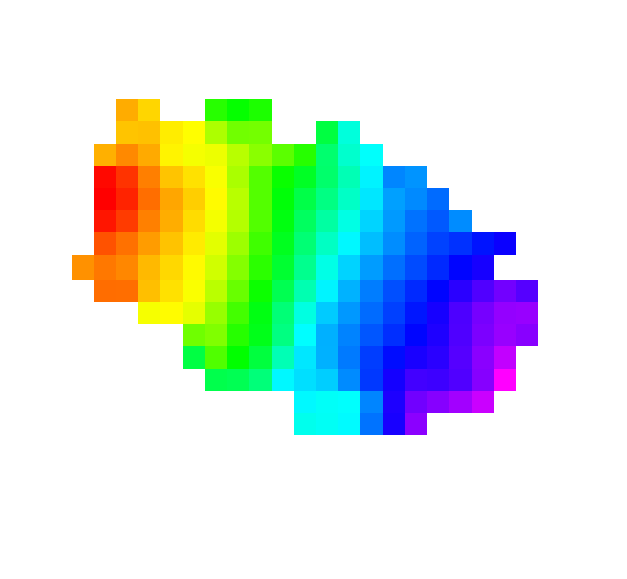
\includegraphics[width=0.6\linewidth]{{graphics/VelManual}.eps}
	\end{textblock*}
	
	%horizontal arrow and text
	\begin{textblock*}{5cm}(4.5cm,3cm)
		\centering
		\hspace{-10pt}
		Automatic \\
		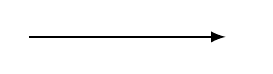
\begin{tikzpicture}[thick]
			\draw [black,   -latex      ] (0,7.0) -- (2.5,7.0) node [right] {};
		\end{tikzpicture}
	\end{textblock*}
	
	%vertical arrow
	\begin{textblock*}{5cm}(7.7cm,4.2cm)
		\centering
		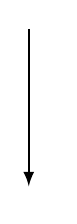
\begin{tikzpicture}[thick]
			\draw [black,   -latex      ] (0,9.0) -- (0.0,7.0) node [right] {};
		\end{tikzpicture}
	\end{textblock*}
	
	%vertical text
	\begin{textblock*}{5cm}(6.5cm,5.2cm)
		\centering
		Manual
	\end{textblock*}
	
	%three spectra
	\begin{textblock*}{7cm}(1cm,6.5cm)
		\centering
		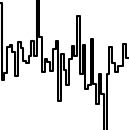
\includegraphics[width=0.25\linewidth]{{graphics/BadSpectrum}.png}
		\hfill
		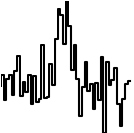
\includegraphics[width=0.25\linewidth]{{graphics/MediumSpectrum}.png}
		\hfill
		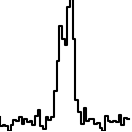
\includegraphics[width=0.25\linewidth]{{graphics/GoodSpectrum}.png}
	\end{textblock*}	
	
	%arrow for bad spectrum
	\begin{textblock*}{5cm}(-0.3cm, 4.3cm)
		\centering
		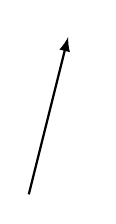
\begin{tikzpicture}[thick]
			\draw [black,   -latex      ] (0,7.0) -- (0.5,9) node [right] {};
		\end{tikzpicture}
	\end{textblock*}
	
	%arrow for medium spectrum
	\begin{textblock*}{5cm}(1cm, 3.9cm)
		\centering
		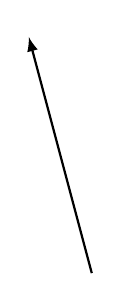
\begin{tikzpicture}[thick]
			\draw [black,   -latex      ] (0.8,7.0) -- (0,10) node [right] {};
		\end{tikzpicture}
	\end{textblock*}
	
	%arrow for medium spectrum
	\begin{textblock*}{5cm}(2.5cm, 3.3cm)
		\centering
		\begin{tikzpicture}[thick]
			\draw [black,   -latex      ] (4.5,7.0) -- (1,10.5) node [right] {};
		\end{tikzpicture}
	\end{textblock*}
	
	
\end{frame}



\begin{frame}{Kinematical modelling}
	\framesubtitle{Fitting a model}
	
	\begin{columns}
		\begin{column}{0.3\linewidth}
			Use a ramp model with a \textcolor{red}{linear internal variation} and a \textcolor{blue}{plateau}.
			
			\hspace*{-10pt}
			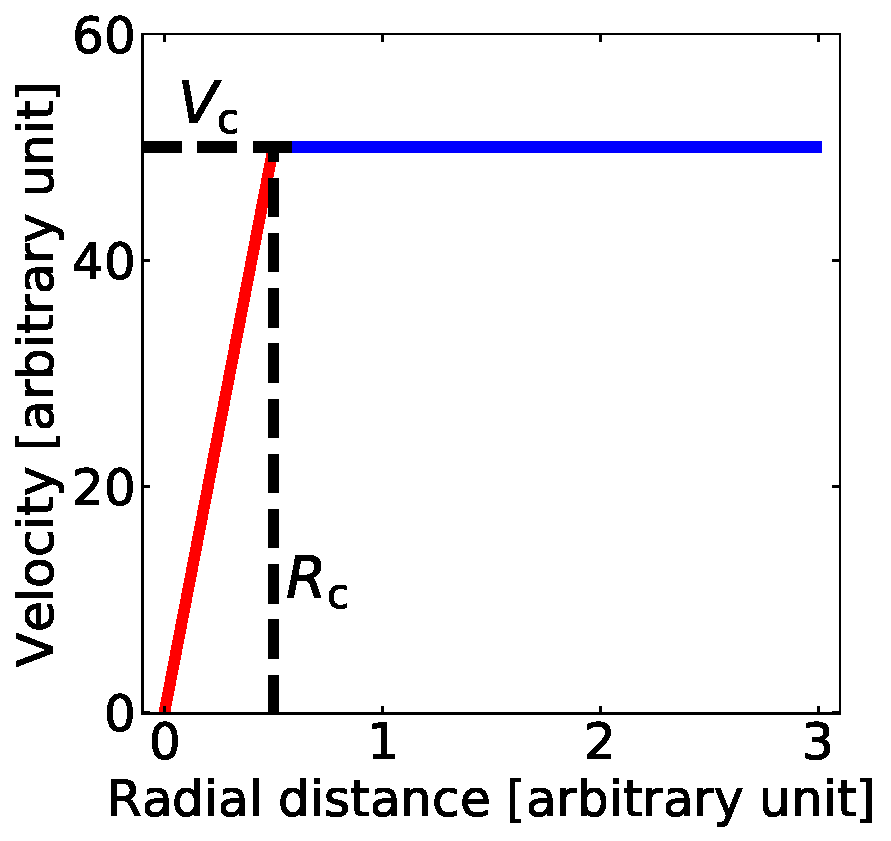
\includegraphics[width=1.3\linewidth]{{graphics/ramp_model}.pdf}
			
		\end{column}	
	
		\begin{column}{0.8\linewidth}
			\centering
			\hspace*{5pt}
			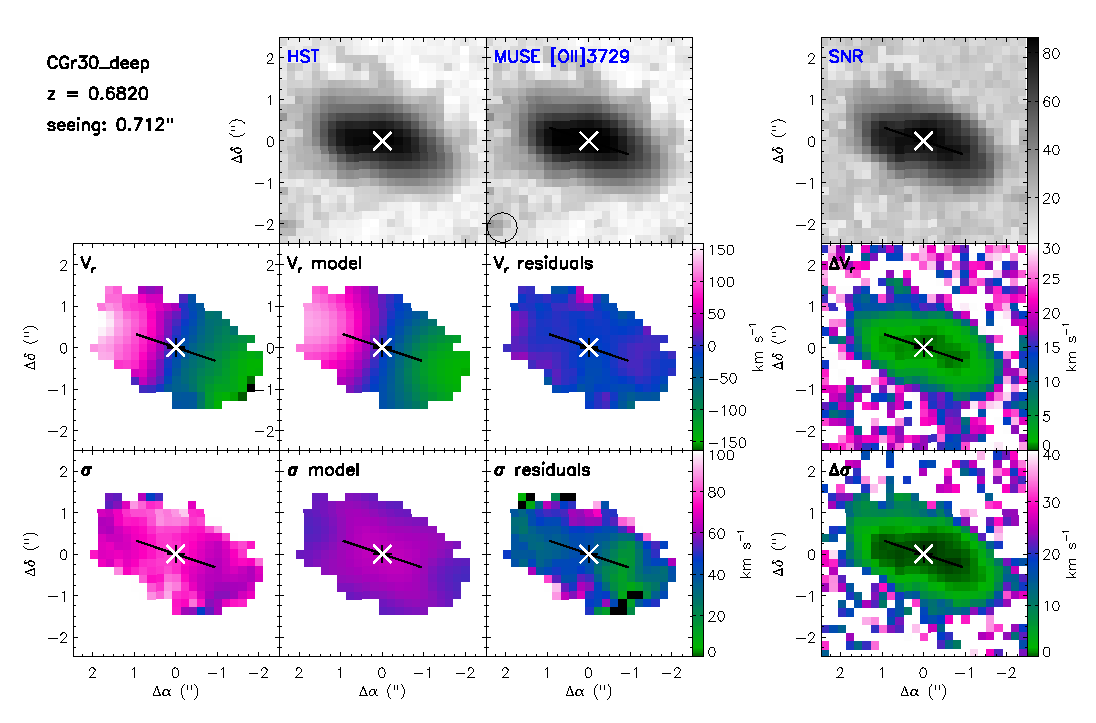
\includegraphics[width=\linewidth]{{graphics/maps_CGr30_deep_91_o2_paper}.eps}
		\end{column}
	\end{columns}
\end{frame}


\begin{frame}{Kinematics of edge-on galaxies}
	
	\begin{columns}
		\begin{column}{0.6\linewidth}
			\centering
			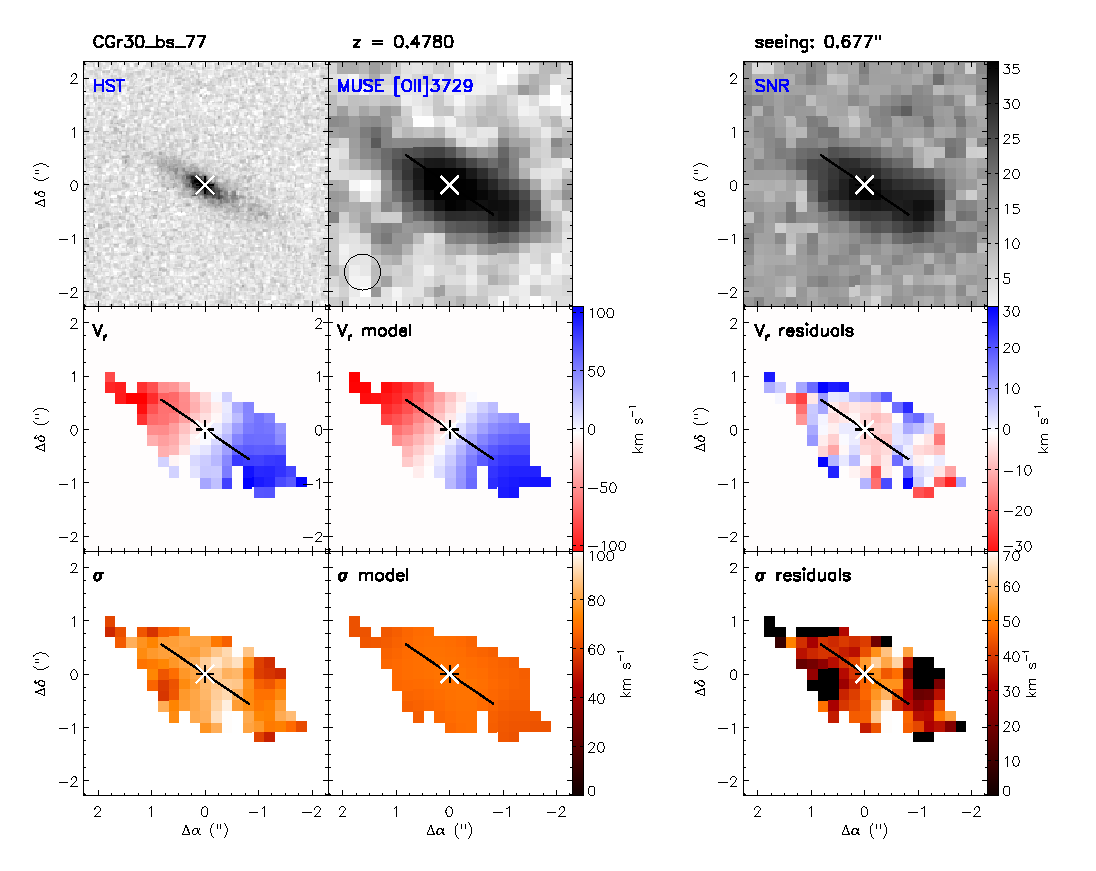
\includegraphics[width=\linewidth]{{graphics/maps_CGr30_bs_77_o2_paper}.eps}
		\end{column}
			
		\begin{column}{0.6\linewidth}
			\centering
			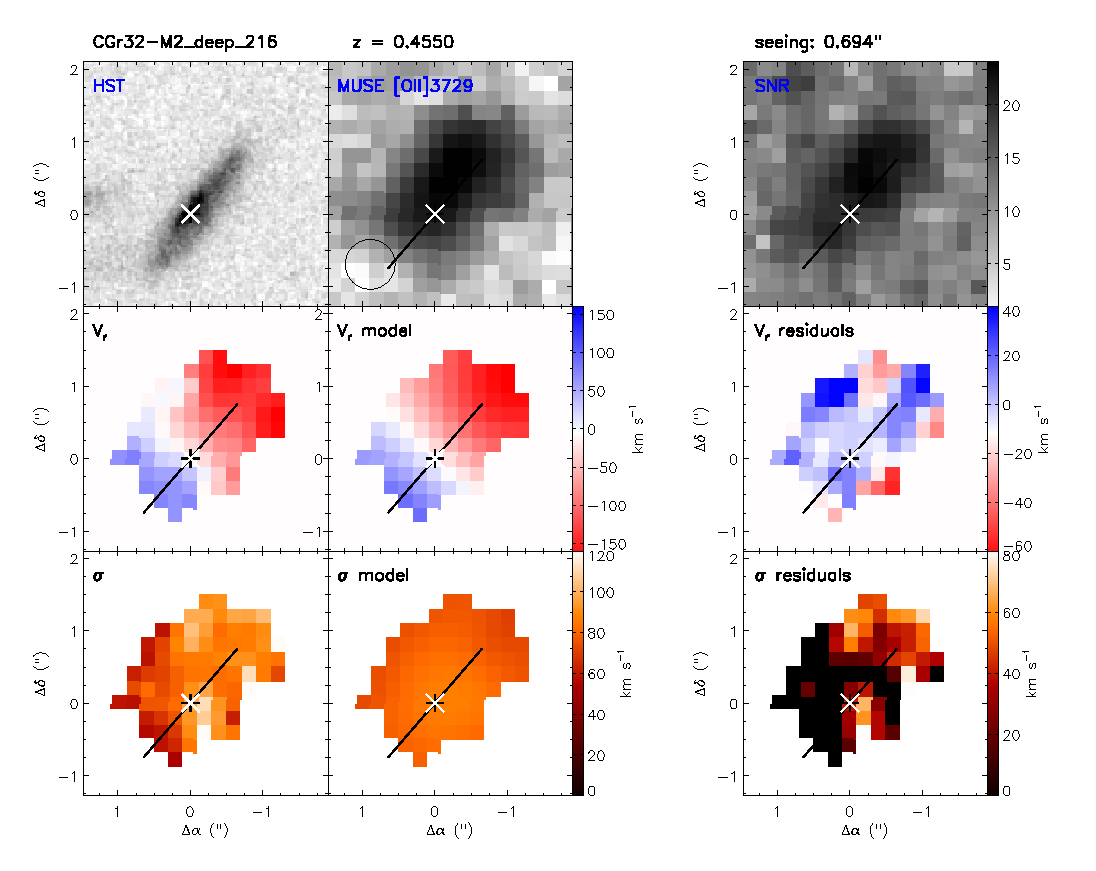
\includegraphics[width=\linewidth]{{graphics/maps_CGr32-M2_deep_216_o2_paper}.eps}
		\end{column}
	\end{columns}
	
	\begin{textblock*}{11cm}(2.5cm, 8cm)
		$i \approx 74 \degree$
	\end{textblock*}
	
	\begin{textblock*}{11cm}(9cm, 8cm)
		$i \approx 72 \degree$
	\end{textblock*}
	
\end{frame}



\begin{frame}{Limitations for small galaxies}
	
	\begin{columns}
		\begin{column}{0.8\linewidth}
			\centering
			\vspace{-15pt}
			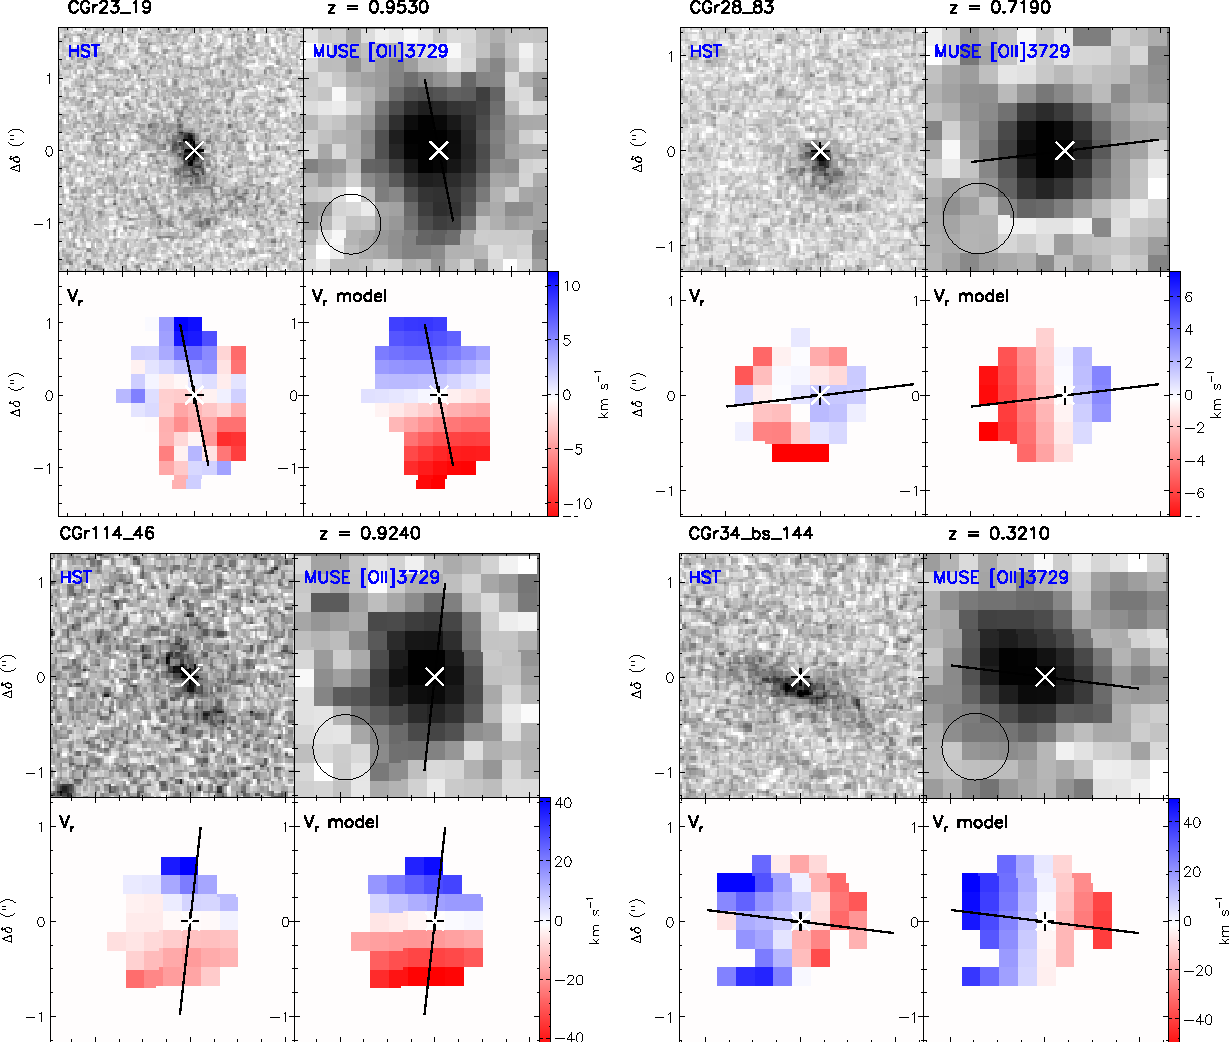
\includegraphics[width=\linewidth]{{graphics/low_size_maps_paper}.pdf}
		\end{column}
		
		\begin{column}{0.3\linewidth}
			\begin{itemize}[label=$\rhd$]
				\item Small and low SNR galaxies tend to have perturbed kinematics
			\end{itemize}
		\end{column}
	\end{columns}
\end{frame}



\begin{frame}{Interacting galaxies ?}
	\begin{columns}	
		\begin{column}{0.9\linewidth}
			\centering
			\hspace*{-10pt}
			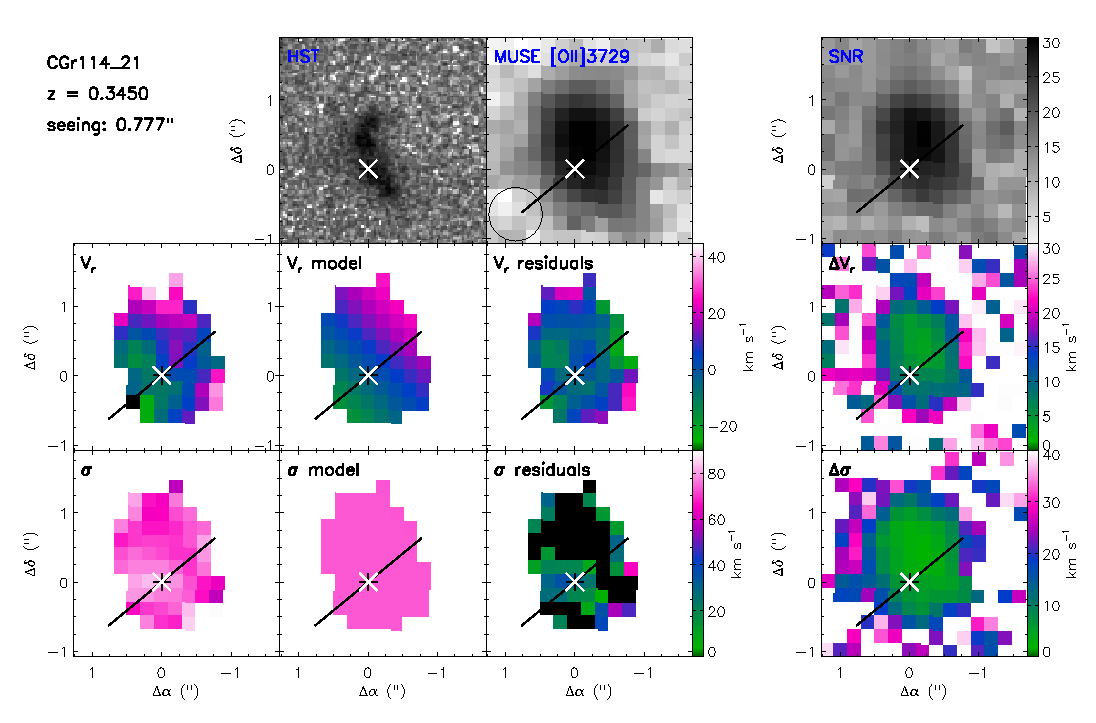
\includegraphics[width=\linewidth]{{graphics/maps_CGr114_21_o2_paper}.eps}
		\end{column}
		
		\hspace*{-10pt}
		\begin{column}{0.3\linewidth}
			
			\begin{itemize}[label=$\rhd$]
				\item Clumpy structure is lost in MUSE whitelight
				\item But \textbf{velocity field is highly perturbed}
				\item Clumps separated by $\approx 3 \rm{kpc}$
				\item Interacting galaxies ?
			\end{itemize}
		\end{column}	
	\end{columns}
\end{frame}





\begin{frame}{A few preliminary results}
	\framesubtitle{Tully-Fisher Relation}
	\centering{
	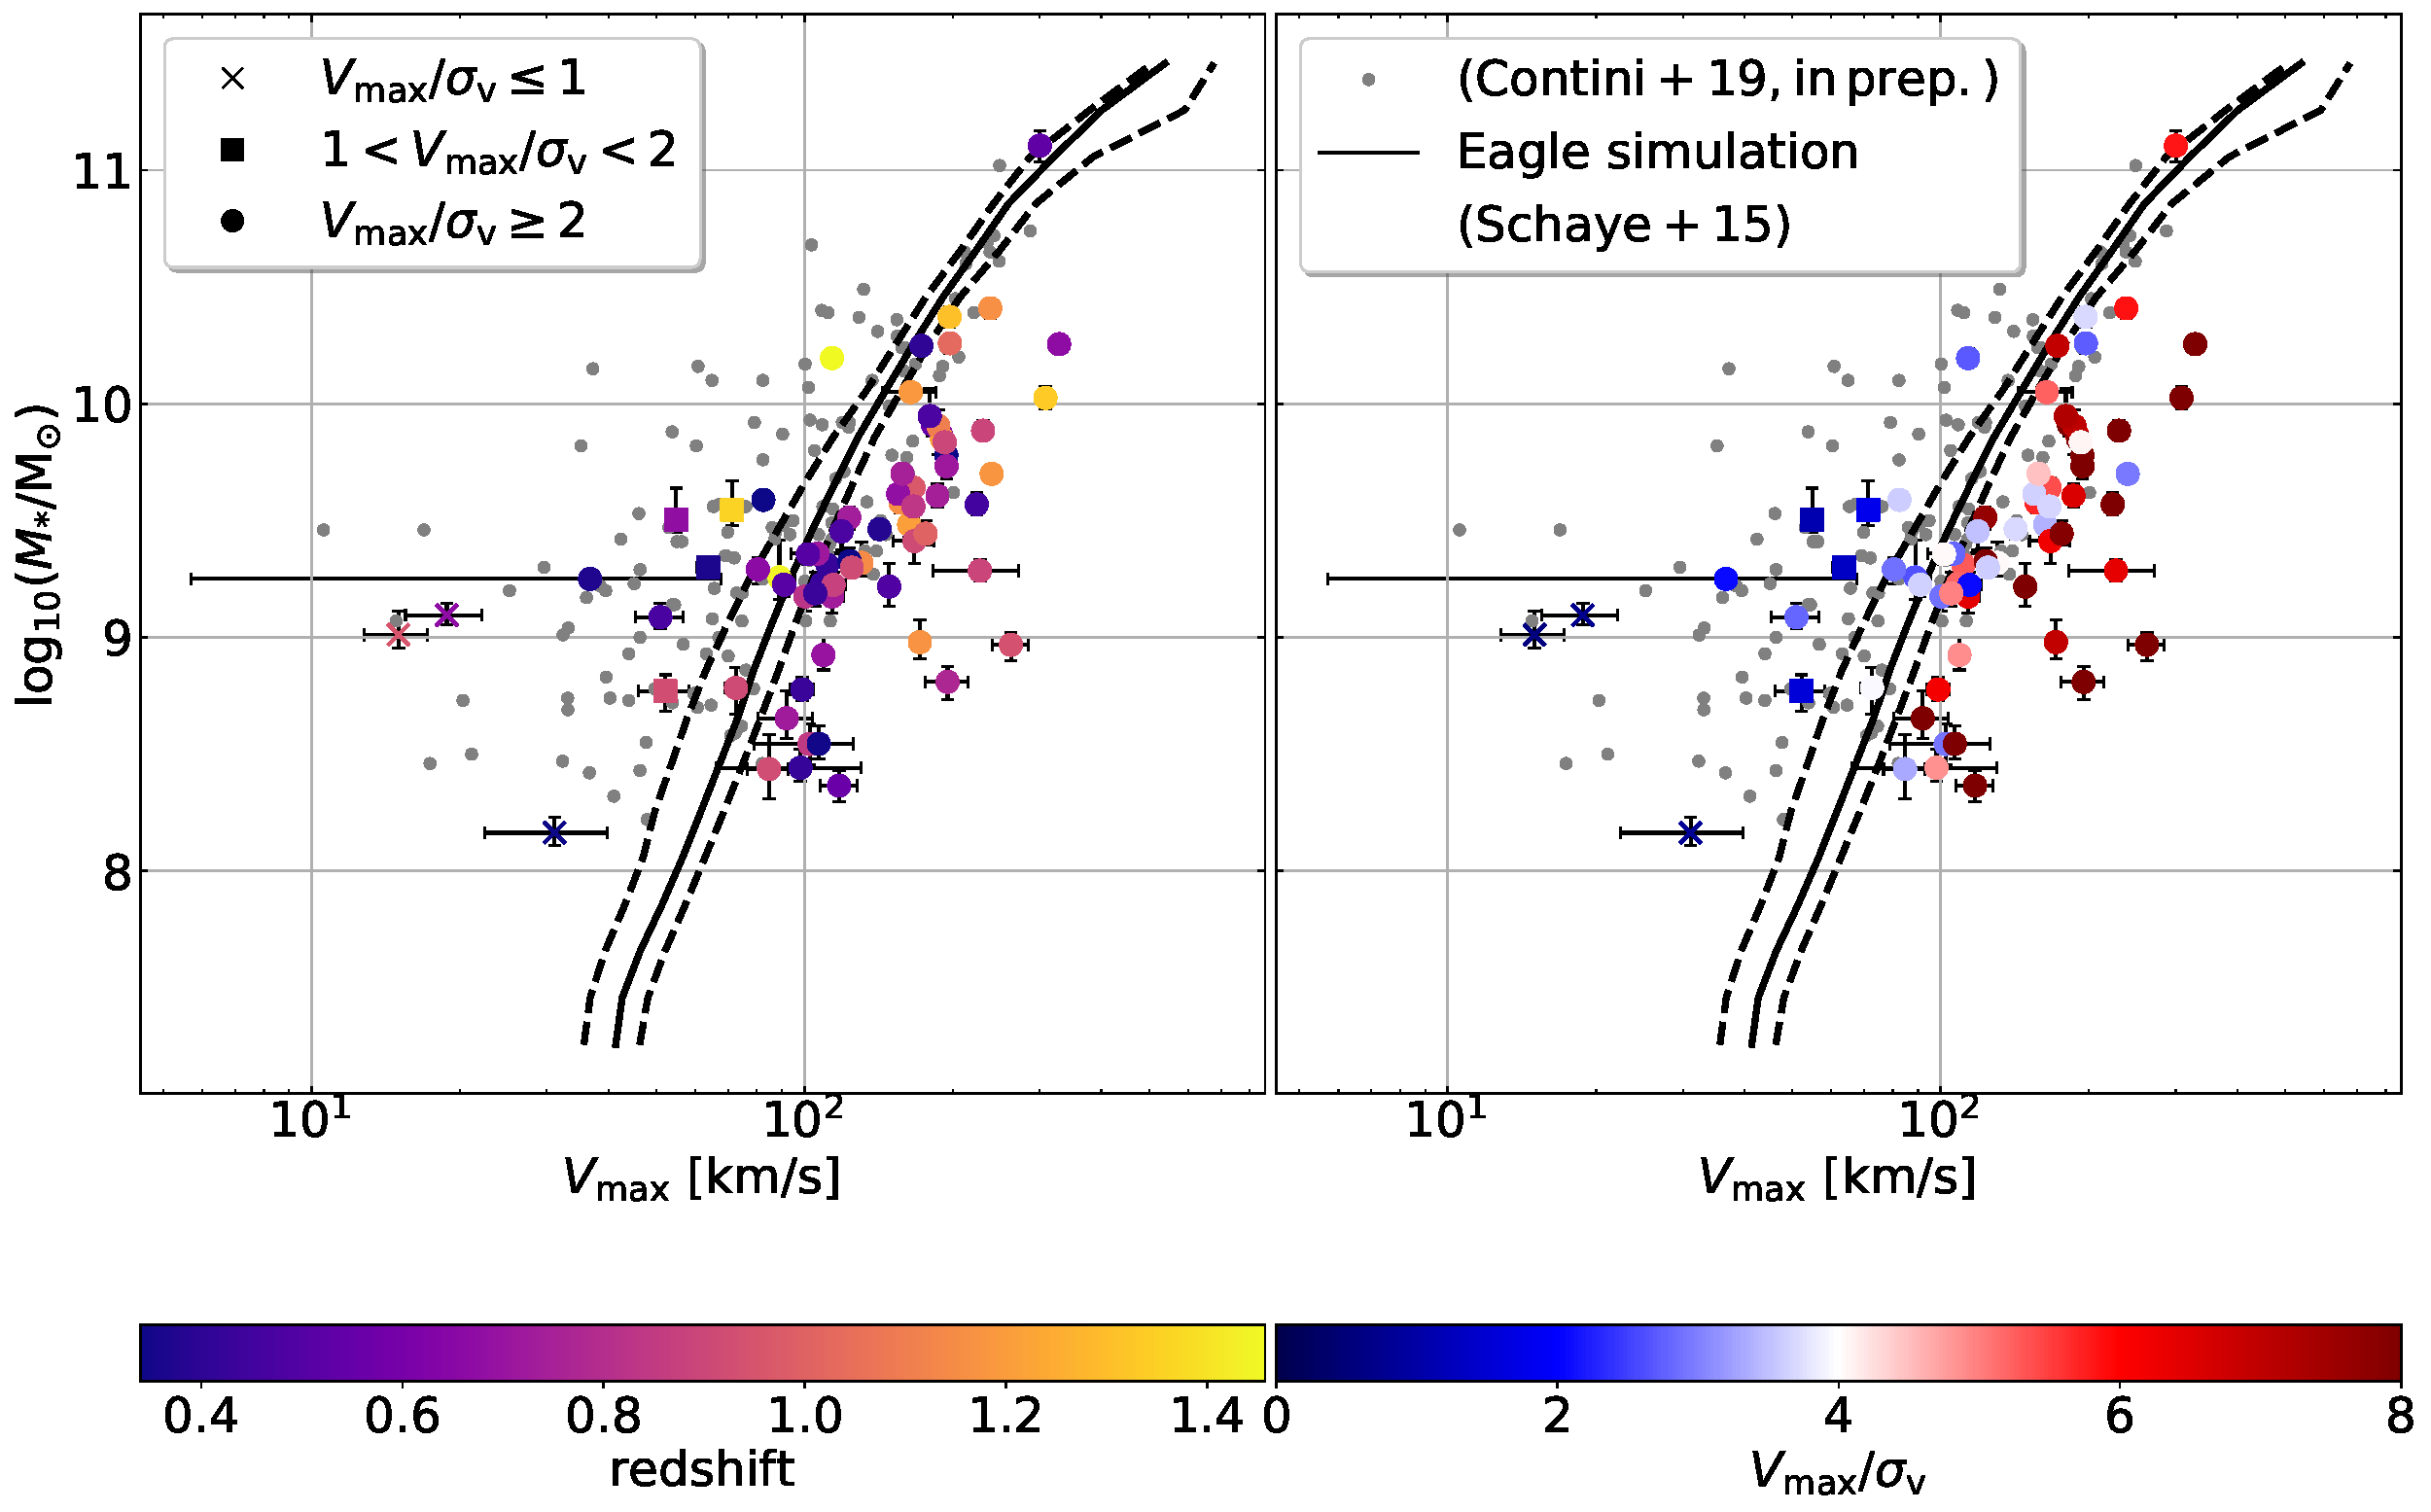
\includegraphics[width=0.9\linewidth]{{graphics/TFRz}.pdf}}
	
	\vspace{-5pt}	
	
	\begin{itemize}[label=$\rhd$]
		\item \textbf{higher $\mathbf{V_{\rm{max}}}$} than in MUSE sample in HUDF of Contini et al. (2019) and EAGLE simulation
		\item \textbf{no} evolution with redshift found
	\end{itemize}
\end{frame}



\begin{frame}{A few preliminary results}
	\framesubtitle{A correlation between $\rm{SFR}$ and $\sigma_{\rm{v}}$ ?}
	
	\begin{columns}	
		\begin{column}{0.6\linewidth}
			\centering
			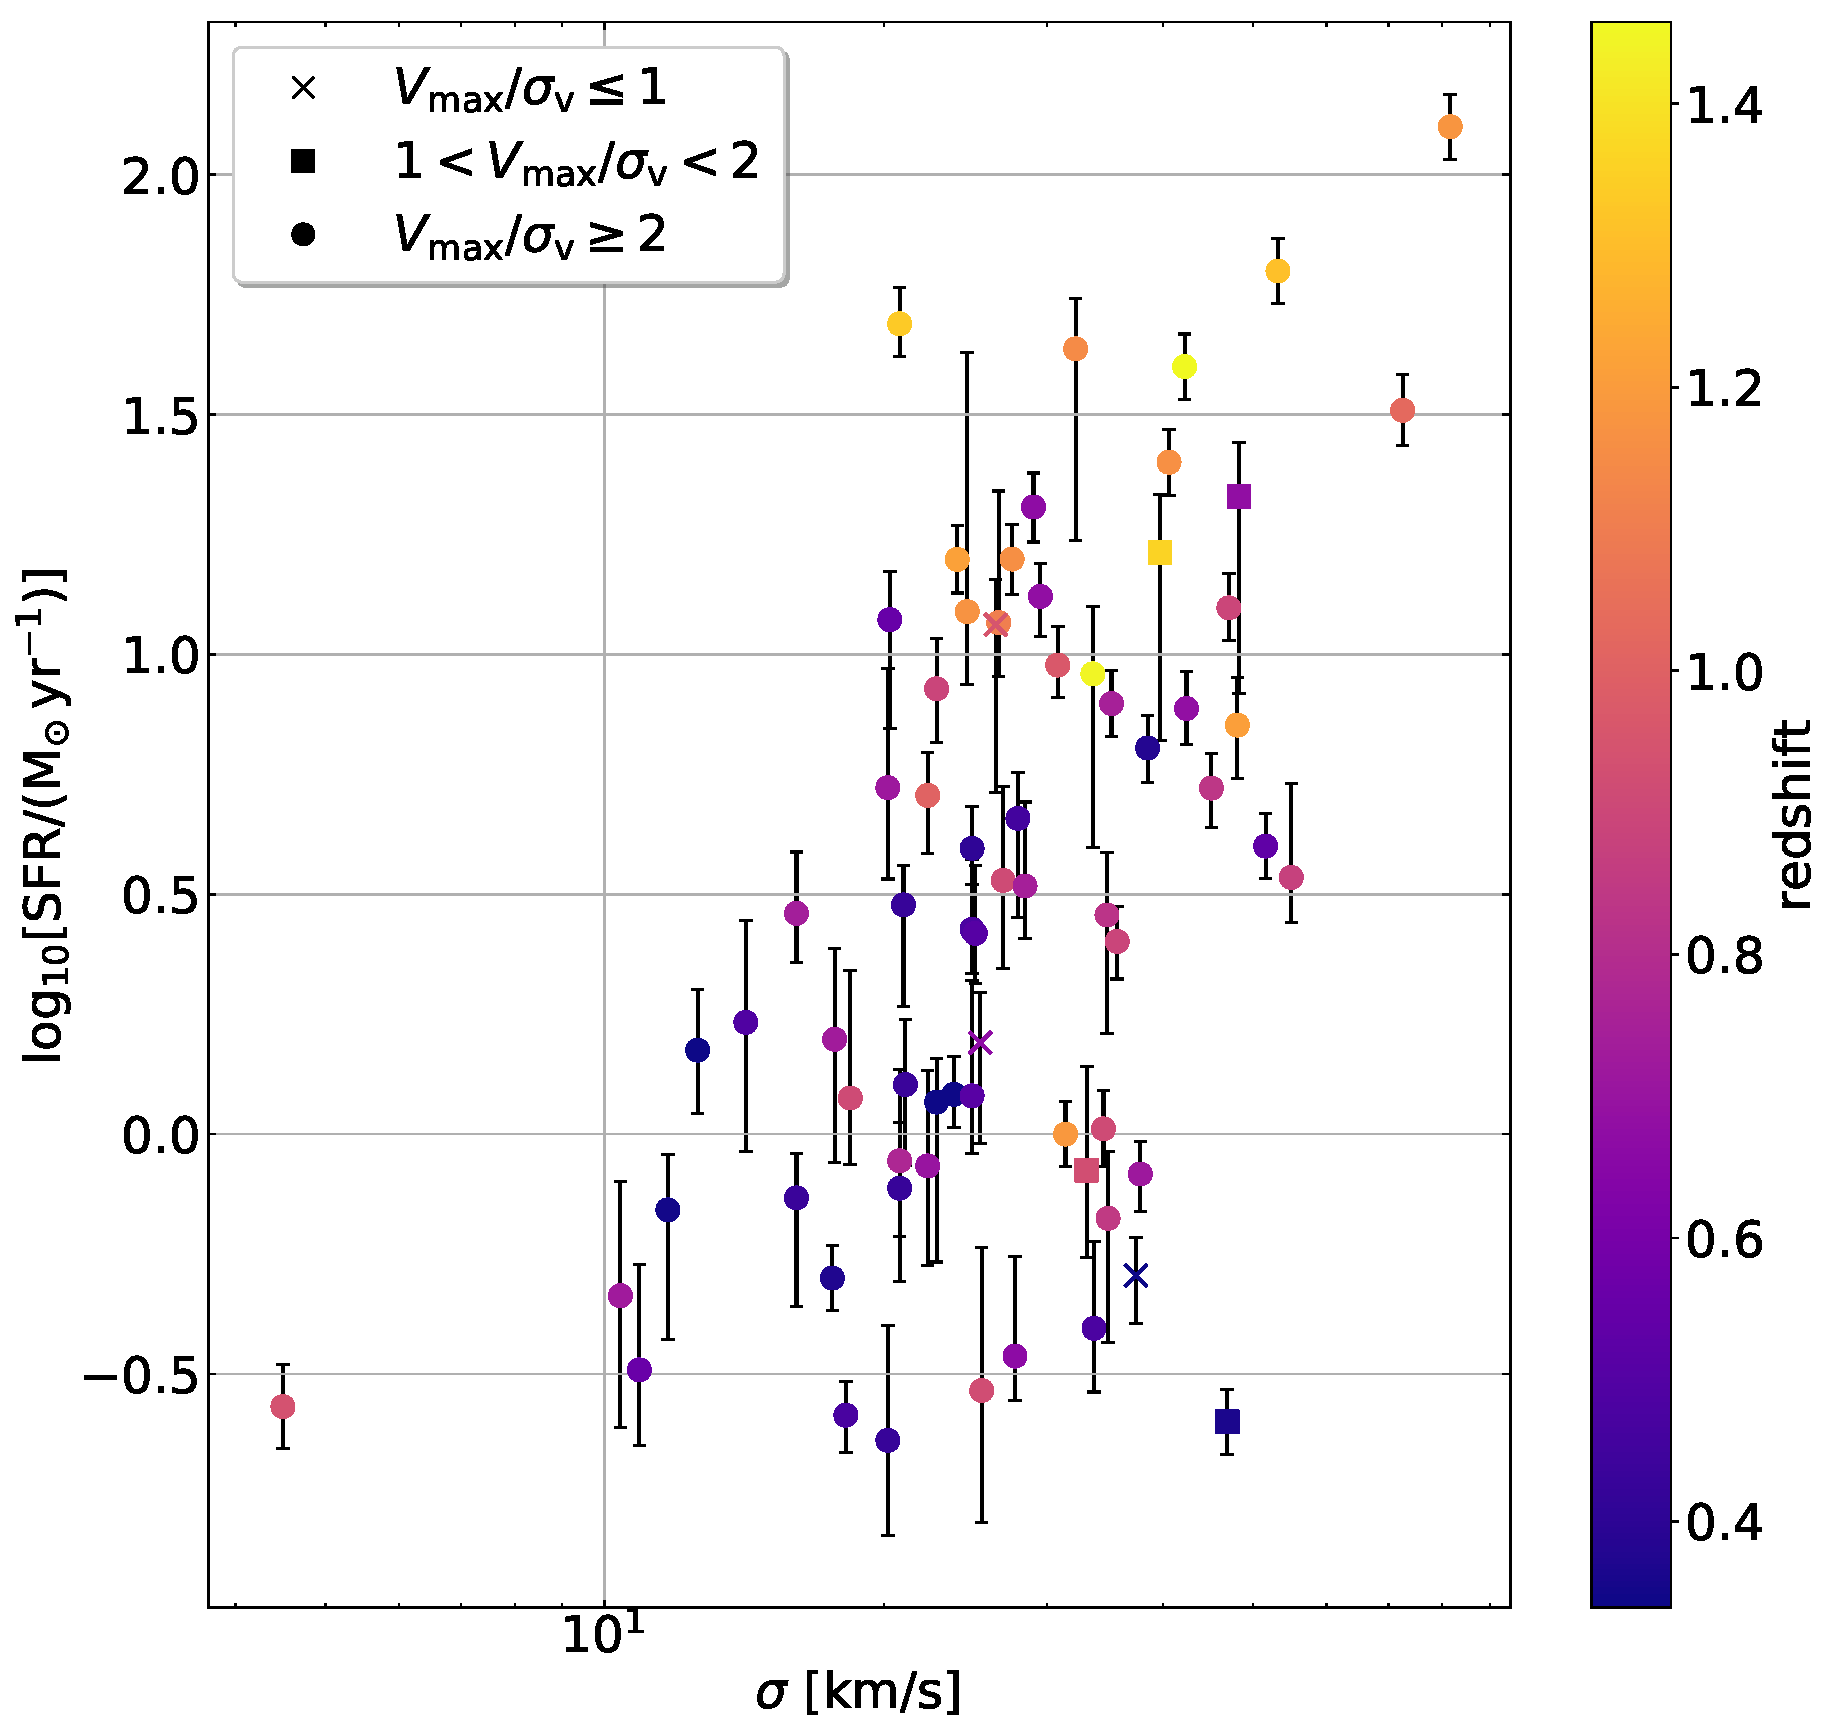
\includegraphics[width=\linewidth]{{graphics/SFR_sigma}.pdf}
		\end{column}
		\begin{column}{0.5\linewidth}
			Correlation between $\mathbf{\rm{SFR}}$ and
			\begin{enumerate}[label=(\alph*)]
				\item \textbf{redshift} $\rightarrow$ consistent with mass-$\rm{SFR}$ relation
				\item \textbf{velocity dispersion}
			\end{enumerate}
			
			\vspace{25pt}
			
			Origin ? \\
			According to Lehnert et al. (2013), energy injection from star-formation.
		\end{column}
	\end{columns}
\end{frame}



\begin{frame}{Perspectives}
	\framesubtitle{Long term (PhD)}

	\begin{columns}
		\begin{column}{0.8\linewidth}
			\begin{itemize}[label=$\rhd$]
				\item \textbf{better selection + larger sample (x10)}
				\item Improve morphological \\ modelling
				\item Angular momentum \\ evolution ?
				\item Dark matter vs. luminous \\ mass ?
				\item \textbf{Very deep} observations + \textbf{stacking} \\ $\rightarrow$ explore dark matter distribution at large radii
			\end{itemize}
		\end{column}		
	\begin{column}{0.48\linewidth}	
	\begin{textblock*}{3.5cm}(9cm, 1.5cm)
		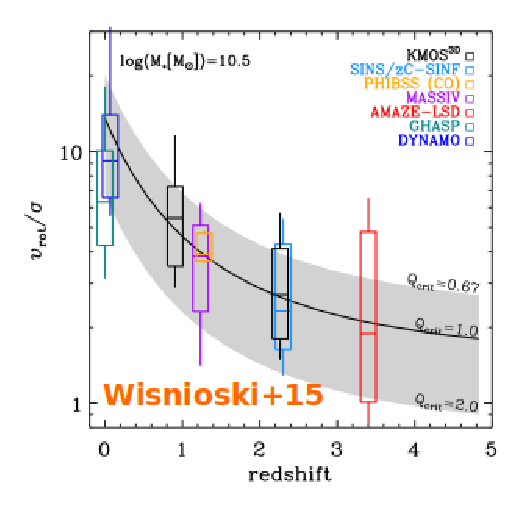
\includegraphics[width=\linewidth]{{graphics/V_sigma_autre_papier}.eps}
	\end{textblock*}
	
	\begin{textblock*}{3.5cm}(9cm, 5.5cm)
		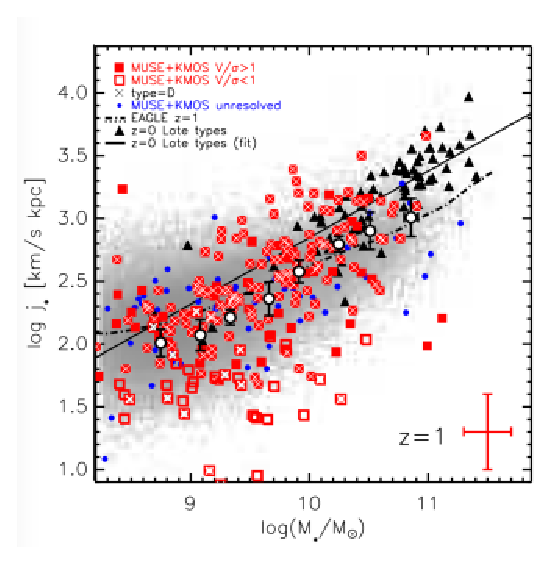
\includegraphics[width=\linewidth]{{graphics/angular_momentum_evolution}.eps}
	\end{textblock*}
	
	\begin{textblock*}{2.5cm}(9.5cm, 5.3cm)
		\textbf{\textcolor{orange}{Swinbank+17}}
	\end{textblock*}
	
	\begin{textblock*}{3.5cm}(6cm, 3.5cm)
		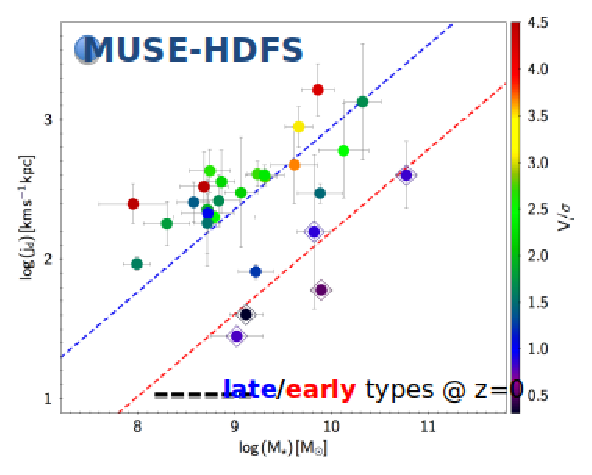
\includegraphics[width=\linewidth]{{graphics/angular_momentum_evolutionCONTINI}.eps}
	\end{textblock*}
	
	\begin{textblock*}{3.5cm}(6.3cm, 5.5cm)
		\textbf{\textcolor{orange}{Contini+16}}
	\end{textblock*}
	
	\end{column}
	\end{columns}
\end{frame}


\end{document}











